\documentclass[titlepage,a4paper,12pt]{book}

\usepackage[utf8]{inputenc}
\usepackage[catalan]{babel}
\usepackage{graphicx}
\usepackage{marvosym}

\begin{document}

\thispagestyle{empty}
%PAGINA3
\rule{160mm}{0.20mm}\\
\textbf{DADES DEL PROJECTE}\\
\\
\textit{Títol del Projecte:} Algoritmes genètics aplicats a ciències de la vida\\
\\
\\
\textit{Nom de l'estudiant:}Raimon Grau Cuscó\\
\\
\textit{Titulació:} Enginyeria Informàtica\\
\\
\textit{Crèdits:} 37.50 \\
\\
\textit{Director/Ponent:} Ignasi Belda Reig / Jordi Delgado Pin\\
\\
\textit{Departament:} Llenguatges i Sistemes Informàtics\\
\\
\\
\rule{160mm}{0.20mm}\\
\textbf{MEMBRES DEL TRIBUNAL}\textit{(nom i signatura)}\\
\\
\textit{President:} Jordi Torres Viñals.\\
\\
\\
\textit{Vocal:} Juan Luis Esteban Ángeles.\\
\\
\\
\textit{Secretari:} Eduardo Ayguadé Parra.\\
\\
\\
\\
\rule{160mm}{0.20mm}\\
\textbf{QUALIFICACIÓ}\\
\\
\textit{Qualificació numèrica:}\\
\textit{Qualificació descriptiva:}\\
\\
\textit{Data:}
\\
\\
\rule{160mm}{0.20mm}\\
%end pagina3
\newpage{\pagestyle{empty}\cleardoublepage}
%PORTADA AMB FOTOS I TAL SINÓ FORA
\begin{titlepage}
\begin{center}
{\Huge Algorismes genètics aplicats a ciències de la vida}\\[2cm]
{\Large  Raimon Grau Cuscó }\\[5cm]

	\begin{figure}[h]
	\begin{center}
	%\includegraphics[width=4in]{img/ip.eps}
	\end{center}
	\end{figure}

	\begin{figure}[h]
	\begin{center}
	%\includegraphics[width=3in]{img/bsc.eps}
	%\includegraphics[width=1in]{img/gridSS.eps}
	\end{center}
	\end{figure}
\end{center}
\end{titlepage}

\newpage{\pagestyle{empty}\cleardoublepage}

\pagenumbering{roman}

%INICIEM
\tableofcontents

\newpage{\pagestyle{empty}\cleardoublepage}

%Introducció
\chapter{Introducció}
\pagenumbering{arabic}
%\addcontentsline{toc}{chapter}{Introducció}
	\documentclass[a4paper]{article}
\usepackage[catalan]{babel}
\usepackage[utf8]{inputenc}
\begin{document}
La computació evolutiva és un camp recerca dins de la informàtica.  Com el nom
indica, es un camp especial dins la computació, una manera determinada d'atacar
problemes que agafa idees en la evolució natural de les espècies.  No es extrany
que s'hagin intentat portar idees de la naturalesa a camps de la computació, i
menys a camps relacionats amb la inteligència artificial, ja que és ben clar
que, la evolució en aquets cas, ha tingut un fort impacte positiu en les
espècies, a nivell individual, i als ecosistemes, amb multitud d'espècies
convivint i co-evolucionant al llarg del temps.

Un altre cas on s'intenta adaptar els procediments naturals en la computació és,
per exemple, en les ``Xarxes neuronals'', on s'intenta simular les interaccions
de les neurones en un cervell, per a solucionar problemes on hi intervé
l'aprenentatge.

fault-tolerance

En general, els problemes que la evolució intenta solucionar (la evolució no
s'atura, amb el qual mai arriba a un estadi totalment estàtic), els soluciona
mitjançant prova i error.

% TODO : Petita intro a la evolució? 

\section{Breu Història} % (fold)
\label{sec:Breu Historia}

Els principis de la aplicació de les idees de Darwin a la resolució de problemes
daten dels anys quaranta, cuan Alan Turing va proposar ``búsquedes genètiques o
evolutives''.  Al any 1962, Bremermann va executar amb èxit alguns experiments
de ``optimització mitjançant evolució i recombinació''.  Durant els anys
seixanta, es van desenvolupar diferents estudis i implementacions d'aquests
principis en 3 llocs diferents, amb 3 noms lleugerament diferents:


 % theme=Berlin;caption_top=1;caption=Els inicis
 % Nom & Qui & On
 % Fogel, Owens, Walsh & programació evolutiva & EEUU
 % & Algoritme genètic & Holanda
 % Rechenberg, Schwefel & estratègies evolutives & Alemanya

\begin{table}
\centering
\caption{Els inicis}
\begin{tabular}{|l|l|l|}
\hline
\multicolumn{1}{|c|}{\textbf{Nom }} & \multicolumn{1}{c|}{\textbf{ Qui }} & \multicolumn{1}{c|}{\textbf{ On}} \\
\hline
\hline
Fogel, Owens, Walsh  & programació evolutiva  & EEUU     \\
                     & Algoritme genètic      & Holanda  \\
Rechenberg, Schwefel & estratègies evolutives & Alemanya \\
\hline
\end{tabular}
\end{table}

Més endavant, als anys noranta, John Koza va encunyar el terme programació
genètica.  Actualment, totes aquestes variants es conceben dins del que
s'anomenen algorismes evolutius.

% TODO : Ferreira i GEP

Avui dia, i donat que les cerques en problemes NP-Complets son més i més
rellevants, les tècniques englobades dins dels algorismes evolutius estan tenint
cada any més rellevància.  Prova d'això és que ja hi ha vàries conferències
i publicacions dedicades.

\subsection{Inspiració de la Naturalesa} % (fold)
\label{sub:Inspiracio de la Naturalesa}

\subsubsection{Evolució darwiniana} % (fold)
\label{ssub:Evolucio darwiniana}

La teoria de la Evolució de Darwin \cite{Darwin} dóna una explicació de la
diversitat biològica i dels mecanismes de sel·lecció natural.  Aquesta
sel·lecció natural és qui juga el paper principal en la direcció que agafa la
evolució.  Donat un entorn que pot assumir un número limitat de individus, i
l'instint bàsic dels individus a reproduir-se, la sel·lecció esdevé inevitable.
Altrament, la població s'aniria incrementat indefinidament, i l'entorn no podria
suportar-ho.  La sel·lecció natural fa que els individus competeixin pels
recursos existents, i permet només reproduir-se als que estiguin més adaptats al
medi en qüestió.

\subsubsection{Genètica} % (fold)
\label{ssub:Genetica}

% subsubsection Genetica} (end)

% subsubsection Evolucio darwiniana (end)

% subsection Inspiració de la Naturalesa (end)

\section{Introduccio als Algorismes evolutius} % (fold)
\label{sec:Introduccio als AE}

% section Introduccio als AE (end)
% section Breu Història (end)

\section{Estat de l'art} % (fold)
\label{sec:Estat de l'art}

Actualment, els algorismes genètics estan essent més i més utilitzats no sols en
el món acadèmic, sinó també en el món de l'empresa.  Per exemplificar això, es
presenten les dades d'un article publicat a 
%XXX 

Les últimes publicacions referents a algorismes genètics tendeixen cap a
optimitzacions de la convergència, i moltes de les tècniques aprofiten sistemes
distribuits



\subsection{Tecnologia} % (fold)
\label{sub:Tecnologia}

Des dels inicis de la programació 'moderna', el llenguatge per excelència
relacionat amb la Intelligència artificial ha estat \cite{LISP}, creat per John
Macarthy el 1958 donat la gran flexibilitat que oferia (a més, en auqells temps
hi havia fortran com a alternativa, un llenguatge molt més rígid).  Així doncs,
els majors avenços relacionats amb la IA han tingut gairebé sempre les seves
primeres implementacions en lisps o derivats (scheme).  

El problema de llenguatges tant dinàmics com lisp, és que al treballar sobre
màquina virtual (lisp es va poder compilar a partir del %XXX
) i eren massa lents per a la implementació en producció.  Recordem que les
aplicacions que utilitzen algorismes de intelligència artificial requereixen un
gran volum de càlculs.

És per això que els sistemes amb grans necessitats de càlcul per a producció
normalment s'implementen amb llenguatges ``propers al ferro'' com poden ser
C/C++. 

Actualment i donada la gran potència de calcul dels ordenadors actuals, hi ha
empreses que comencen a utilitzar llenguatges interpretats per a realitzar
algorismes genètics  com per exemple \footnote{oblong}.
% subsection Tecnologia (end)

% section Estat de l'art (end)
\end{document}

\chapter{Algoritmes genètics}
	%
%        File: pholus.tex
%     Created: Wed Jul 08 02:00 PM 2009 C
% Last Change: Wed Jul 08 02:00 PM 2009 C
%
\documentclass[a4paper]{article}
\usepackage[spanish]{babel}
\usepackage[utf8]{inputenc}
\begin{document}

\section{Algoritmes Evolutius}\label{sec:ae}

L'aplicació de regles evolutives en problemes de computació va començar en els
anys %XXX 
amb Goldberg

\begin{itemize}
\item Goldberg
\item Koza
\item Ferreira
\item 
\item 
\item 

\end{itemize}

\subsection{Problemes a atacar}\label{sub:problemes a atacar}

El tipus de problemes més adequats per a solucionar amb Algorismes evolutius,
són desde problemes d'optimització, problemes que no sabem a què responen, i
problemes on evolucionen els propis programes.  Aquest últim tipus de problemes,
també són coneguts més específicament com algorismes genètics.  En aquest
projecte, un dels casos a tractar s'ha solucionat utilitzant una modificació
d'algoritme genètic

\end{document}

	%\include{genetics}

\chapter{BedRoc Tanimotos}
%\documentclass[titlepage,a4paper,12pt]{report}

\usepackage[latin1]{inputenc}
\usepackage[catalan]{babel}
\usepackage[dvips]{graphicx}
\usepackage{marvosym}
\usepackage{amsmath, amsthm, amssymb}
\usepackage{graphicx}
%\usepackage{hyphenat}
\usepackage{longtable}
\usepackage{setspace}
%\usepackage{a4wide}
%\usepackage{babel}
%\usepackage{tocbibind}
%\usepackage{cite}
%\usepackage{subfigure}
%\usepackage{multirow}

\begin{document}

\title{Projecte Final de Carrera-no tinc t�tol encara}
\author{Xavier Maresma Coll}
\date{\today}
\maketitle
\pagenumbering{arabic}

\tableofcontents  %%Index

\part{Semblances entre molecules}

\chapter{Introducci� qu�mica al problema}
%Introducci� qu�mica sobre lo dels potencials, la semblan�a i aquestes coses

Aquest projecte consistir� en explicar el proc�s que ens ha portat fins a considerar les M�quines de Suport Vectorial com la millor t�cnica per a la discriminaci� en el cas en qu� ens trobem. Per aix� abans de comen�ar, explicarem el context qu�mic en el que ens mourem. 

Aquest treball forma part de la nova tecnologia desenvolupada per Intelligent Pharma, anomenada HELIOS, que serveix per identificar,a partir d'un compost de refer�ncia pr�viament donat, nous compostos amb propietats estructurals completament diferents que imiten el comportament d'aquest compost de refer�ncia. Per exemple, si el compost de refer�ncia ja �s conegut (per exemple, un extret d'un producte natural o d'una patent), HELIOS pot trobar compostos no  vinculats estructuralmnt que reprodueixin les seves propietats psico-qu�miques tridimensionals; per tant, aquests compostos tindran les mateixes caracter�stiques biol�giques per� amb diferent estructura mol�lecular. A aquesta b�squeda se l'anomena "Scaffold hopping" (b�squeda entre diferents fam�lies qu�miques).

La t�cnica utilitzada �s el Virtual Screening(VS), que normalment s'utilitza per descobrir noves fam�lies qu�miques en relaci� a una activitat biol�gica desitjada. El VS t� m�todes que es basen en l'estructura dels compostos i d'altres que no. Com hem dit, HELIOS t� com a objectiu identificar nous compostos que no s�n an�legs estructuralment, per� s� biol�gicament. 

HELIOS es basa en la superposici� de camps mol�leculars entre qualsevol compost i un lligam de refer�ncia. Per� HELIOS, no nom�s considera la superposici� generada per c�rregues formals, sin� tamb� altres tipus relacionades amb el comportament din�mic; aix�, es fan diferents superposicions entre parells de mol�l�cules es duen a terme a la vegada. 
L'alineament de camps mol�leculars va ser descrit durant els anys noranta, per� no s'ha dut a terme fins aquesta d�cada degut a que l'alineament mol�lecular flexible �s un problema impossible de resoldre sense les eines de supercomputaci�. Fins els �ltims anys, el Virtual Screening basat en els lligams s'ha basat en metodologies per buscar semblances moleculars com l'estructura, farmac�for, etc. 

HELIOS utilitza alineaments de camps moleculars flexibles per identificar compostos que s'assemblin a un compost de refer�ncia. L'alineament molecular e duu a terme mitjan�ant la metodologia "cloud computing", la qual permet fer-ho en pocs dies. Els compostos amb els quals es fa l'alineament es treuen d'una base de dades que pot variar segons l'objectiu de la b�squeda. 

Els camps moleculars s�n discretitzats dins d'una caixa en forma de grid de punts. Idealment, la caixa hauria de ser suficientment gran per introduir-hi tots els lligans de la base de dades en una conformaci� extesa. De la mateixa manera la capsa ha d'incloure aquells punts al voltant de les mol�cules que tenen valors significatius. Diferents representacions dels camps moleculars, que donen diferent informaci� sobre la densitat electr�nica, s�n construits amb sondes at�miques. Una sonda at�mica �s una part�cula amb caracter�stiques qu�miques particulars que s'assemblen a propietats at�miques en ambients electr�nics particulars. 

Les 22 sondes at�miques que s�n implementades en HELIOS s�n les que  es veuen a la taula \ref{table:maps} 

\begin{table}
\centering
\begin{tabular}{|ccc|}
\hline
aromatic carbon &aliphatic carbon&non-hydrogen bonding sulfur\\
non-hydrogen bonding phosphor&phosphor&non-hydrogen bonding nitrogen\\
hydrogen donor&oxygen acceptor&nitrogen acceptor\\
sulfur acceptor&spherical nitrogen acceptor&spherical oxygen acceptor\\
fluorine&chlorine&bromine\\
iodine&iron&manganese\\
calcium&magnesium&zinc\\
positive charge&& \\
\hline
\end{tabular}
\caption{The 22 atom probes implemented in HELIOS.}
\label{table:maps}
\end{table}

El camp molecular definit per una sonda en un punt donat �s calculat amb la seg�ent equaci�

\[
V = C_1 \sum \limits_{i} \left(\frac{A_{pi}}{r_{pi}^{12}}-\frac{B_{pi}}{r_{pi}^{6}}\right)+C_2 \sum \limits_{i} E(t)\left(\frac{C_{pi}}{r_{pi}^{12}}-\frac{D_{pi}}{r_{pi}^{10}}\right)+C_3 \sum \limits_{i}\frac{qi}{\epsilon r{pi}}
\]

on $p$ i $i$ indexen la sonda i l'�tom lligant respectivament, i $A, B, C$ i $D$ s�n par�metres; $E(t)$ �s una funci� de la geometria dels ponts d'hidrogen establerta; $\epsilon$ indica la constant diel�ctrica i $C_{1}$, $C_{2}$ i $C_{3}$ s�n constants.

L'alineament m�ltiple de camps moleculars flexibles �s una taxa complexa que requereix de t�cniques i recursos computacionals avan�ats. El proc�s implementat per HELIOS fixa el camp molecular del compost de refer�ncia i utilitza algoritmes evolutius en un sistems de "cloud-computing" per duu a terme l'alineament flexible m�ltiple dels camps moleculars de cadasc�n dels diferents compostos que hi ha dins la base de dades.

Amb aix� obtenim per a cada mol�l�cula de la base de dades 22 vectors on hi ha els valors per cadasc�n dels punts ordenats del grid de les 22 sondes moleculars. A partir d'aqu� hem de trobar alguna manera d'evaluar la similitud entre mol�l�cules.

\chapter{�ndex de semblan�a}

Fins ara tenim el seg�ent: una base de dades de mol�l�cules que hem d'ordenar segons la semblan�a amb una mol�l�cula de refer�ncia. Per a cada mol�cula considerem la discretitzaci� del camp molecular (grid o capsa) ordenada de manera que tinguem les 22 representacions del grid en 22 vectors on a la posici� $i$ del vector hi vagi el valor del punt del grid que estigui en la posici� $i$ segons l'ordenaci� que hem considerat. Per tant, el seg�ent pas seria determinar num�ricament una mesura de la semblan�a entre els grids (vectors). Abans de fer aquest pas, repassem diferents conceptes importants i algunes mesures que seran candidates a evaluar la semblan�a en el nostre problema.

La idea de determinar una mesura num�rica de la semblan�a entre dos objectes, cadascun caracteritzats per un conjunts d'atributs, �s com� de moltes disciplines, com biologia,psicologia, recuperaci� d'informaci� bibliogr�fica. Per tant, considerarem a partir d'ara el cas general de buscar semblances entre dos vectors. 

En general, semblan�a $S_{A,B}$ entre dos objectes �s estimada pel nombre d'elements iguals que tenen. Els objectes que s�n iguals, haurien de tenir la m�xima puntuaci�. Per tant, una expressi� de la semblan�a seria en termes de la teoria de conjunts, la intersecci� $(A\cap B)$ que en l�gica seria l'operador $AND$. La dissimilitud $D_{A,b}$ �s estimat pel nombre d'elements diferents que tenen. Els objectes id�ntics obtindrien la m�nima puntuaci�. An�logament a la similitud, parlant en termes de teoria de conjunts, la dissimilitud es calcularia posant amb la uni� $(A\cup B)$ o el que seria el mateix amb l'operador l�gic $OR$. El denominador ser� simplement un normalitzador per tenir l'�ndex entre 0 i 1. 

El concepte de semblan�a normalment s'utilitza per referir-se tan a la semblan�a com a la difer�ncia, ja que es suposa que si dos objectes s�n semblants �s perqu� no s�n diferents. En matem�tiques i estad�stica s'utilitzen els conceptes de semblan�a, proximitat, dist�ncia per referir-se al mateix, per� en qu�mica similitut i dissimilitut poden portar a diferents resultats. Per exemple, considerem dues seq��ncies de car�cters, F1 i F2, cadascuna t� conjunts de 407 car�cters, 402 dels quals s�n comuns entre ells. F3 i F4, cadascuna t� un conjunt de 5 car�cters, dels quals cap d'ells �s com�. En els dos casos la dist�ncia Eucl�dia �s $10 \over 1024$  o $0.0098$ quan �s evident que les dues primeres s�n m�s semblants entre elles que la segona parella.

\section{Mesures}
 
Alguns dels coeficients s�n mesures de les dist�ncies o dissimilitut entre objectes (i tenen valor 0 per objectes id�ntics), mentre que altres mesures semblances directament(i tenen el valor m�xim per objectes id�ntics). En la majoria els coeficients de mesura estaran entre 0 i 1 o poden ser normalitzats, la qual cosa vol dir que estan fitats tan superiorment com inferiorment. Aquest rang entre 0 i 1 permet a partir d'una mesura obtenir la seva complement�ria, cosa que en alguns casos de similitut ha passat que paral�lelament s'han desenvolupat dues mesures que s'ha vist que eren complementaries, per� que tenien diferents noms. 

Els coeficients de dist�ncia s�n an�legs a una dist�ncia en un espai geom�tric multidimensional, tot i que no necess�riament han de ser equivalents. Recordem el concepte dist�ncia, perqu� una dist�ncia sigui considerada com una m�trica ha de complir el seg�ent:

\begin{enumerate}
\item $D_{A,B}\geq 0$,  $D_{A,A}=D_{B,B}=0$
\item  $D_{A,B}=D_{B,A}$
\item $D_{A,B} \leq D_{A,C} + D_{C,B}$ 
\item $A\neq B \Longleftrightarrow D_{A,B} > 0$
\end{enumerate}

Una dist�ncia que compleixi les tres primeres propietas se l'anomena una pseudom�trica i si no compleix la tercera tampoc se l'anomena una no-m�trica. Per� que un coeficient de dist�ncia compleixi les quatre propietats, no vol dir que es pugui fer un embedding a un espai euclidi�, es requereixen altres propietats. 

De coeficients se n'han definit molt, tan de similitut com de dist�ncia, per� molts d'ells s'ha demostrat que estan relacionat o simplement molt correlacionats. Per aix�, mostrarem coeficients que no estiguin correlacionats. 

\subsection{Mesures qualitatives}

Suposem que els valors estan restringits a 0 i 1. En aquest context cal definir un nombre de s�mbols que poden ser importants. Primerament, caracteritzem dos objectes A i B com $X_{A}$ i $X_{B}$, llavors definim:
\begin{center}
$a=\sum_{j=1}^{j=n} x_{jA}$	nombre de 1's en A

$b=\sum_{j=1}^{j=n} x_{jB}$     nombre de 1's en B

$c=\sum_{j=1}^{j=n} x_{jA}x_{jB}$   nombre de 1's en A i B a la vegada

$d=\sum_{j=1}^{j=n} (1-x_{jA}-x_{jB}+x_{jA}x_{jB}$ nombre de 0's en A i B a la vegada

\end{center}

I d'aquesta manera, tenim $n=a+b-c+d$. Aquestes quantitats representen conjunts ($a=\mid\chi_{A}\mid$, $b=\mid\chi_{B}\mid$, $\mid\chi_{A}\cap\chi_{B}\mid$, $d=n-\mid\chi_{A}\cup\chi_{B}\mid$), i la igualtat final s'aconsegueix simplement aplicant la teoria de conjunts ($\mid\chi_{A}\cup\chi_{B}\mid=a+b-c$).

A partir d'aqu� es poden construir diferents mesures intuitivament. A les taules \ref{tablemesures} i \ref{tablemesures2} es mostren, expressades de manera diferent, les principals mesures de similitut, dissimilitut i mixtes, tot i que algunes d'aquestes que es poden fer servir s�n el producte d'una mesura de similitut amb una de dissimilitut, com Dixon que utilitzava el producte d'un Tanimoto amb una dist�ncia eucl�dia. 

\begin{table}
\centering
\begin{tabular}{|c|c|c|}
\hline 
Tipus & Nom de la mesura & mesura qualitativa\\ \hline
\multirow{4}{4cm}{Mesures de Similitut} & nombre d'encerts comuns & c \\ 
\cline{2-3}
&Tanimoto & $c/(a+b-c)$\\ 
\cline{2-3}
&Dice & $2c/(a+b)$\\ 
\cline{2-3}
&Cosinus,Carbo & $c/(ab)^{2}$\\
\hline
\multirow{2}{4cm}{Mesures de Dissimilitut} & distancia Hamming & a+b-2c\\
\cline{2-3}
&distancia eucl�dea & $\sqrt{(a+b-2c)}$\\
\hline
\multirow{2}{4cm}{mesures mixtes} & Hamann & $(3c+d-a-b)/(a+b+d-2c)$\\
\cline{2-3}
& Tversky & $\rho c - \alpha a - \beta b$ \\
\hline
\end{tabular}
\caption{Tipus de Mesures}
\label{tablemesures}
\end{table}

\begin{table}
\centering
\begin{tabular}{|c|c|c|}
\hline
Tipus & Nom de la mesura &  definici� te�rica\\ \hline
\multirow{4}{4cm}{Mesures de Similitut} & nombre d'encerts comuns & $\chi_{A} \cap \chi_{B}$\\
\cline{2-3}
&Tanimoto & $ \mid\chi_{A}\cap\chi_{B}\mid / \mid\chi_{A}\cup\chi_{B}\mid$\\
\cline{2-3}
&Dice & $2[\mid\chi_{A}\cap\chi_{B}\mid]/[\mid\chi_{A}\mid+\mid\chi_{B}\mid]^{1/2}$\\ 
\cline{2-3}
&Cosinus,Carbo & $\mid\chi_{A}\cap\chi_{B}\mid/[\mid\chi_{A}\mid \mid\chi_{B}\mid]$\\
\hline
\multirow{2}{4cm}{Mesures de Dissimilitut} & distancia Hamming & $\mid\chi_{A}\cup\chi_{B}\mid-\mid\chi_{A}\cap\chi_{B}\mid$\\
\cline{2-3}
&distancia eucl�dea & $ [\mid\chi_{A}\cup\chi_{B}\mid-\mid\chi_{A}\cap\chi_{B}\mid]^{1/2}$\\
\hline
\end{tabular}
\caption{Tipus de Mesures}
\label{tablemesures2}
\end{table}


\subsection{Mesures quantitatives}

En aquest cas nom�s fa falta definir $X_{A}$ com el vector de dades de l'objecte A i $X_{B}$ el de B i traduir directament de l'expressi� del coeficient en termes de la teoria de conjunts, ja que $X_{A}X_{B}$ seria equivalent a la intersecci� i $X_{A}+X_{B}-X_{A}X_{B}$ la uni�. 


A la taula \ref{tablemesures2} es mostren mesures pel cas quantitatiu en qu� els valors s�n reals. Les expressions de la dist�ncia eucl�dea i el cosinus s�n els mateix que un espai euclid� de dimensi� finita. 

Apuntar que en el cas l�mit s'hauria de substituir els sumatoris per la integral. 


\begin{table}
\centering
\begin{tabular}{|c|c|c|}
\hline
Tipus & Nom de la mesura & mesura quantitativa \\ \hline
\multirow{4}{4cm}{Mesures de Similitut} & nombre d'encerts comuns & $\sum_{j=1}^{n} X_{jA}X_{jB}$ \\
\cline{2-3}
&Tanimoto & $[\sum_{j=1}^{n} X_{jA}X_{jB}] \over [\sum_{j=1}^{n} (X_{jA})^{2} + \sum_{j=1}^{n} (X_{jB})^{2} + \sum_{j=1}^{n} (X_{jA})(X_{jB})]$ \\
\cline{2-3}
&Dice & $[2\sum_{j=1}^{n} X_{jA}X_{jB}] \over [\sum_{j=1}^{n} (X_{jA})^{2} + \sum_{j=1}^{n} (X_{jB})^{2}]$ \\
\cline{2-3}
&Cosinus,Carbo & $[\sum_{j=1}^{n} X_{jA}X_{jB}] \over [\sum_{j=1}^{n} (X_{jA})^{2} \sum_{j=1}^{n} (X_{jB})^{2}]$ \\
\hline
\multirow{2}{4cm}{Mesures de Dissimilitut} & distancia Hamming & $\sum_{j=1}^{n} |X_{jA}-X_{jB}|$ \\
\cline{2-3}
&distancia eucl�dea & $[\sum_{j=1}^{n} (X_{jA}-X_{jB})^{2}]$ \\
\hline
mesures mixtes & Pearson & $[\sum_{j=1}^{n} (X_{jA}-\bar{X_{jA}})(X_{jB}-\bar{X_{jB}})] \over [\sum_{j=1}^{n} (X_{jA}-\bar{X_{jA}})^{2} \sum_{j=1}^{n} (X_{jB}-\bar{X_{jB}})^{2}$ \\

\hline
\end{tabular}
\caption{Tipus de Mesures2}
\label{tablemesures2}
\end{table}

\subsection{Elecci� de la mesura}

Amb les definicions dels apartats anteriors es descriuen un nombre de coeficients de dist�ncia i similitut que m�s s'usen en el context qu�mic, tan amb variables cont�nues com discretes. 

Entre tots els coeficients de dist�ncia i similitut n'hi ha molts d'ells que estan relacionats. En alguns casos es pot obtenir un coeficient com a combinaci� d'alguns altres; i en d'altres casos coeficients que s�n diferents quan es calculen de manera cont�nua, esdevenen equivalents per atributs discrets. Alguns coeficients se'ls descriu com a monotonics entre ells, que significa que es pot demostrar anal�ticament que sempre produeixen el mateix tipus de ranking tot i calcular-se de forma diferent, d'altres en canvi no seran monotonics per� s� que estaran molt correlacionats. Finalment haurem de triar entre els grups de coeficients que presentin correlacions baixes, el qual voldr� dir que estaran reflexant caracter�stiques diferents dels objectes a evaluar. 

Analitzant les diferents mesures, arribem a la conclusi� que les mesures de similitut s�n monot�niques o correlacinades entre elles (Tanimoto i Dice monot�niques entre elles i correlacionades amb el cosinus) de la mateixa manera que les de dist�ncia (Eucl�dea i de Hamming s�n monotoniques). Les dist�ncies Hamming i Eucl�dea formen part d'una classe dist�ncies anomenades de Minkowski que tenen com a f�rmula general $D_{A,B}=[\sum_{j=1}^{j=n} (|x_{jA}-x_{jB}|)^{t}]^{1/t}$, on $t=1$ �s per la dist�ncia de Hamming i $t=2$ per la dist�ncia Eucl�dea.

Una difer�ncia fonamental entre les dist�ncies de Hamming i Eucl�dea per una banda i els coeficients de Tanimoto, Dice o Cosinus per l'altra, �s que els primers consideren l'abs�ncia d'informaci� (o valors baixos en el cas continu) com una evid�ncia de similitut, mentre que l'altre no. Aquest �s un aspecte filos�fic molt discutit en la literatura. Un exemple seria el comentat per Sokal and Sneath: ''L'abs�ncia d'ales entre un grup d'organismes seria un indicador absurd (camells, cavalls, gossos,...). De la mateixa manera la pres�ncia d'ales tamb� podria un mal indicador (rat penat, oreneta, papallona).''

En el context qu�mic les dist�ncies Hamming i Eucl�dea  s�n �tils nom�s per comparacions relatives (entre dues mol�cules semblants) per� no per comparacions absolutes (entre dues mol�cules independents) per les que �s millor coeficients com el de Tanimoto. No obstant, la dist�ncia eucl�dea �s la que s'utilitza en m�todes de clustering, els quals han donat bons resultats.

Una altra difer�ncia fonamental �s que les mesures d'associaci� tenen un factor normalitzador que ajuda a reduir el biaix produit per la mida de les mol�cules. Aix�, si busquem les semblances, una mol�cula gran �s, a priori, m�s probable que tingui m�s elements en com� que una mol�cula petita. Si utilitzem mesures de dissimilitud, tenim el problema invers. �s m�s probable que una mol�cula petita tingui menys elements diferents que una mol�cula gran. Per aquest motiu, hi ha estudis on han utilitzat mesures que s�n combinacions de mesures de similitut i dissimilitut, per exemple, Tanimoto amb la dist�ncia Hamming.

Segons Willet, estudis recents en qu� han comparat ambd�s coeficients per veure qui mesurava millor un valor d'activitat equivalent a veure quin era el m�s semblant a un compost de refer�ncia. En aquest estudi els coeficients de similitut han donat millors resultats que els de dissimilitut, sobretot el de Tanimoto i el Cosinus. Per� si s'ha d'escollir un dels dos s'elegeix el de Tanimoto ja que �s m�s r�pid de calcular. 

Un altre criteri que hem descrit �s el d'utilitzar mesures de similitut asim�triques o mixtes basades en la mesura de Tversky. La forma general d'aquesta mesura �s: $S_{A,B}={c \over \alpha(a-c) + \beta(b-c) + c}$ on $\alpha$ i $\beta$ s�n par�metres a definir per l'usuari. Si $\alpha$ i $\beta$ s�n iguals el coeficient resultant �s sim�tric. Si $\alpha=\beta=1/2$ �s iguals al coeficient Dice i si $\alpha=\beta=1$ �s igual al de Tanimoto. Si $\alpha$ i $\beta$ s�n diferents el coeficient resultant ser� asim�tric, i quan  $\alpha=1$ i $\beta=0$ $S_{A,B} = {c \over a}$ que es pot interpretar com la part de A que est� a B. Diferents tipus de mesures s'obtenen amb la modificaci� dels par�metres $\alpha$ i $\beta$.

Finalment ens hem quedat amb el coeficient de Tanimoto com a mesura de la semblan�a entre mol�l�cules. En el seg�ent apartat, explicarem l'adaptaci� d'aquest coeficient al nostre cas. 

Com a conclusi� s'ha de dir que existeixen altres coeficients d'altres disciplines i que no est� demostrat que existeixi un �nic coeficient que sigui el millor. El que s'ha fet en aquest apartat triar els que podrien anar millor, i d'aquests agafar el que �s menys cost�s. 

\subsection{Adaptaci� al nostre cas}

Com hem dit a l'apartat anterior, hem seleccionat el coeficient de Tanimoto. El coeficient de Tanimoto �s definit com la mida de la interesecci� dividida per la mida de la uni� dels conjunts de mostra. Si A i B s�n dos conjunts, en termes de la teoria de conjunts el coeficient de Tanimoto �s igual a 

$$T(A,B)={|A\cup B| \over |A\cap B|}$$

Per tant, si tractem amb vectors el coeficient tindr� la seg�ent expressi�: 

$$T(A,B)={A \cdot B \over \|A\|^{2} + \|B\|^{2} - A�B}$$

Els vectors de dades (de potencials) amb qu� treballem nosaltres pertanyen a $\Re^{N}$ on N s�n el nombre de punts que s'han considerat dins el grid. L'adaptaci� que fem nosaltres �s convertir-los a vectors binaris de manera que nom�s es consideren potencials rellevants. La uni� de dos camps moleculars alineats s�n totes aquells punts de l'espai on qualsevol dels dos camps presentet potencials de Van del Waals menors de -0.1 i el valor absolut del potencial electrost�tic �s m�s gran que 0.5 o amb potencials de desolvataci� m�s grans que 0.25(C'). La intersecci� s�n tots aquells punts de la uni� que presenten difer�ncies entre els camps moleculars m�s petites de 0.25(C). Per tant, el nostre coeficient de Tanimoto modificat �s definit com:

$$T'_{j}(A_{j},B_{j})={C_{j} \over C'_{j}}$$

on j �s un camp molecular donat. Un cop $T'_{j}$ �s calculat per cadasc�n dels 22 camps moleculars, el coeficient de Tanimoto final, $T'_{i}$ (compost de refer�ncia i), �s calculat amb una mitjana aritm�tica ponderada:

$$T'_{i}={\sum_{j=0}^{n} \omega_{j}\cdot T'_{i,j} \over \sum_{j=0}^{n} \omega_{j}}$$

L'�ltim pas va ser trobar una ponderaci� general dels 22 coeficients de Tanimoto. La primera ponderaci� utilitzada va ser trobada sota criteris qu�mics. Llavors es va realitzar un an�lisi de components principals sobre una base dades de 1534 mol�cules i amb una mol�cula de refer�ncia. Els resultats obtinguts van ser millors que amb la ponderaci� sota criteris qu�mics. 

Obtinguts aquests resultats es va agafar la mateixa base de dades i es va calcular els coeficients de Tanimoto amb 10 mol�cules de refer�ncia diferents i es va realitzar un an�lisi can�nica de poblacions per veure si es podia trobar una ponderaci� �nica, i els resultats obtinguts van mostrar que no era possible. Per tant, degut a l'alt cost computacional que tindria fer un an�lisi de components principals per cada c�lcul s'ha optat per mantenir la ponderaci� sota criteris qu�mics, ja que aquesta en global donava millors resultats que la ponderaci� obtinguda per an�lisi de components principals.

La manera com s'ha avaluat cada ordenaci� s'explica en el seg�ent apartat.

\section{Evaluci� de la ordenaci�}

''Virtual Screening'' �s un terme que s'aplica a un tipus de problema que conceptualment �s l'equivalent computacional de ....... screening, o sigui, a on un gran nombre de mostres (mol�l�cules en aquest cas) estan disposades per ser discriminades entre actives i inactives. Per Intelligent Pharma evaluar l'execuci� del VS �s una pr�ctica necess�ria, ja que �s una forma de seleccionar quin m�tode ordena millor. Com hem indicat en l'apartat anterior evaluar el VS ens servir� per comparar entre diferents ponderacions, o sigui, per determinar quina ponderaci� discrimina millor entre mol�l�cules actives i inactives. 

L'�xit en el ''Virtual Screening'' est� en trobar un bon coeficient que assigni bones puntuacions a les mol�cules interessants(normalment definides com a actives respecte a una prote�na) i males puntuacions a les mol�l�cules menys interessants (inactives). Per tant, un virtual screening exit�s posar� a d'alt de tot de la llista ordenada les mol�l�cules actives i despr�s les inactives. 

A partir d'ara el que tenim �s una llista ordenada de mol�l�cules i volem saber si l'ordenaci� obtinguda �s adequada al nostre problema, per tal de poder comparar diferents coeficients i diferents ponderacions. De fet, aix� no es restringeix nom�s al ''Virtual Screening'', �s un problema universal de tots els exercicis de predicci�. Aix� ens pot ajudar a l'hora de trobar aproximacions de la bondad de l'ordenaci�. El problema �s que el Virtual Screening t� una particularitat, i �s que la proporci� d'actius a posar a d'alt de tot de la llista �s molt petita, i pot provocar molt biaix a l'hora de fer la predicci�. Aquest problema en la literatura �s conegut com el ''early recognition problem''. Aquest tema ha estat de gran inter�s en molts �mbits tan acad�mics com de la ind�stria farmac�utica en els �ltims anys. En aquest apartat estudiarem diferents maneres de tractar el problema presentat. 

\subsection{Propietats de les m�triques}

S'ha fet pal�l�s recentment en la literatura que als qu�mics m�dics i computacionals els hi falten m�todes est�ndards o universals per evaluar els resultats d'algun nou assaig. Aquest �s el t�pic indicador d'un camp que ha estat mal desenvolupat. En efecte, hi ha moltes m�triques diferents que estan en �s, a vegades adaptades d'altres camp. Malgrat tot, cap d'aquestes m�triques que s'usen aconsegueix resoldre el problema de ''early recognition'' que �s espec�fic del VS. 

Considerant altres mesures que han esdevingut estandards en altres camps, Nicholls, proposa les seg�ents propietats que hauria de tenir: 

\begin{enumerate}
\item Independ�ncia respecte les variables
\item Robustesa
\item Expressions d'error
\item Abs�ncia de par�metres lliures (sobretot de la proporci� d'actius)
\item F�cil d'entendre i d'interpretar
\end{enumerate}

Per solucionar el problema del ''early recognition'' seria bo que la m�trica diferenci�s entre tres casos: (1)la meitat dels actius es troben al principi de la llista i la resta al final, (2)els actius estan distribuits uniformement al llarg de la llista i (3) tots els actius estan situats al mig de la llista. Una bona m�trica ha els tres casos segons aquest ordre.

A continaci� mostrarem les diferents m�triques que m�s s'utilitzen i mostrarem les seves virtuds i les seves debilitats.

\subsection{M�triques}

\begin{enumerate}
\item �rea sota la curva acumulada(AUAC)

L'AUAC �s simplement l'�rea sota la funci� distribuci� de les mol�l�cules actives. S'utlitza la funci� de distribuci� emp�rica, o sigui, que a l'eix de les abcisses hi ha el rang relatiu de les mol�l�cules (es segueix l'ordre creixen dels rangs, de millora pitjor) i a les ordenades hi ha la proporci� relativa d'actives. Si notem la funci� de distribuci� com $F_{a}(x)$, la qual �s la probabilitat de trobar un actiu en el primer x \% de la mostra, l'AUAC �s obtinguda: 
\begin{center}
$ AUAC=\int_{0}^{1} F_{a}(x) dx$
\end{center}

Aqu�, $F_{a}(x)$ �s normalitzada i per tant va de l'origen al punt $(1,1)$. Al ser una funci� de distribuci� el pitjor valor �s 0 i el millor valor �s 1 i si les les actives estan distribu�des uniformement, el valor esperat de AUAC �s 0.5. Per tant, l'AUAC pot ser interpretat com la probabilitat que un actiu seleccionat d'una mostra on els actius estan distribuits segons la funci� de distribuci� emp�rica de la nostra llista ordenada, estigui millor situat que un actiu seleccionat aleatoriament d'una mostra on el ranking dels actius segueix una funci� de distribuci� uniforme. 

En el cas discret l'AUAC es calcularia de la seg�ent manera:
\begin{center}
$ AUAC={1 \over 2nN}\sum_{k=0}^{n} [F_{a}(k)+F_{a}(k+1)]$
\end{center}

Aqu� $F_{a}(x)$ no est� normalitzada ja que hi ha el coeficient $nN$. Prenem el conveni de que la funci� de distribuci� est� normalitzada impl�citament en el cas continu i expl�citament en el cas discret. Per tant, $F_{a}(k)$ ser� la posici� del k-�ssim actiu trobat a la nostra llista ordenada. El valor m�xim de l'AUAC, quan tots els actius estan al principi de la llista, ser� $1-{n \over (2N)}$ que tendeix a 1 quan ${n\over N}$ es fa petit; el min�m valor �s ${n\over(2N)}$, quan tots els actius estan al final de la llista.

Si considerem $w(x)$ qualsevol funci� cont�nua i suficientment suau en funci� del rang relatiu, podem definir l'�rea sota la corba acumulada ponderada (weighted area under the accumulation curve) calculada: 

\begin{center}
$ wAUAC={\int_{0}^{1} F_{a}(x)w(x)dx \over \int_{0}^{1} w(x)dx}$
\end{center}

Si integrem per parts el numerador
$$\int_{0}^{1}F_{a}(x)w(x)dx=F_{a}(1)F_{w}(1)-F_{a}(0)F_{w}(0)-\int_{0}^{1}F_{w}(x){dF_{a}(x)\over dx}dx$$
$$=F_{w}(1)-\int_{0}^{1}F_{w}(x)f_{a}(x) dx$$

on $f_{a}(x)$ �s la funci� de densitat emp�rica i $F_{w}(x)=\int_{0}^{x}w(z)dz$. Aix� porta a que poguem expressar wAUAC com:
$$wAUAC={F_{w}(1)-\int_{0}^{1}F_{w}(x)f_{a}(x) dx \over F_{w}(1)}$$

Si apliquem una funci� de pesos uniforme $w(x)=1$ llavors $F_{w}(x)=x$ i wAUAC �s igual a AUAC, i podem escriure AUAC de la seg�ent manera:
$$AUAC=1-\int_{0}^{1} xf_{a}(x)dx$$

Aix� AUAC queda en funci� de l'esperan�a del rang relatiu, el que mostra que �s equivalent a aquesta esperan�a, excepte en qu� la interpretaci� del coeficient �s oposada. 

Aquesta expressi� en el cas discret, si considerem que $r_{i}$ �s el rang de l'actiu i-�ssim de la llista i $x_{i}$ el rang relatiu, queda:

$$AUAC=1-{1\over nN}\sum_{i=0}^{n} r_{i} = 1-{1\over n}\sum_{i=0}^{n} x_{i}$$

Notar que en el cas discret existeix un petit error, ja que est� formulat com una integral de Riemann. Aquest error disminueix a mesura que augmenta N. 

Aquesta nova expressi� mostra que un actiu situal al principi o al final de la llista ordenada influeix de la mateixa manera sobre l'AUAC. 

Aquesta m�trica no s'usa molt ja que no distingeix entre els tres casos considerats en l'apartat anterior. 

\item{�rea sota la corba ROC}

La corba de ROC �s una m�trica �mpliament usada en moltes disciplines com l'estad�stica, medicina, criminologia i bioinform�tica. El seu origen est� en l'an�lisi de la detecci� del senyal i ha estat molt utilitzada per la comunitat m�dica per evaluar el poder discriminatori de nombrosos tests. La corba de ROC s'obt� representant el soroll (proporci� de falsos positius) en l'eix de les abcisses contral el senyal (verdaders positius) en l'eix de les ordenades. Si apliquem la corba de ROC en el ''virtual screening'', aquesta il�lustra l'�xit en ordenar les actives (senyal) per davant de les inactives (soroll). La popularitat de la corba de ROC sobre altres m�triques, prov� del fet que �s no param�trica, no necessita cap suposici� sobre la forma de la distribuci�. A m�s, la seva representaci� gr�fica �s molt �til per determinar visulament si l'ordenaci� �s bona o no. L'�rea sota la corba de ROC �s simplement la probabilitat que un verdader positiu (actiu) escollit aleat�riament estigui m�s ben classificat que un fals positiu (inactiu) escollit aleat�riament, el qual est� altament relacionat amb el test de suma de rangs de Wilcoxon. Aquest nombre permet la predicci� de la probable efectivitat d'una eina en l'experiment. Aquesta habilitat predictiva no la t� la m�trica presentada anteriorment, l'AUAC, perqu� mentre la ROC descriu una propietat de l'aplicaci� estudiada, les altres m�triques descriuen una propietat de l'experiment.

La f�rmula de l'�rea sota la corba de ROC en el cas discret �s: 

\begin{center}
$ROC={1 \over nN}\sum_{k=2}^{n} F_{a}(k)[F_{i}(k)-F_{i}(k-1)]$
\end{center}

on $F_{i}(k)$ com per l'AUAC �s la funci� de distribuci� de les mol�cules inactives, la qual en el cas discret no est�normalitzada i per tant, �s la freq��ncia acumulada dels inactius a la posici� k de la llista. $F_{a}(k)$ �s l'an�leg a $F_{i}(k)$ pels actius. 

La definici� de cont�nua de l'�rea sota la ROC �s la seg�ent:

\begin{center}
$ROC=\int_{0}^{1}F_{a}(x)f_{i}(x)dx$
\end{center}

aqu� $f_{i}(x)$ �s la densitat de les inactives dins la llista ordenada. Existeix una terminologia en estad�stica on a $F_{a}(x)$ se l'anomena la sensivitat i a $F_{i}(X)$ 1-l'especificitat. 

L'AUROC t� valors entre 0 i 1. En el cas que totes les actives estan al principi el valor �s 1 i si totes les actives estan al final el valor �s 0. El valor esperat per la corba de ROC en el cas discret si les actives estan distribu�des uniformement �s $1/2+1/[2(N-n)]$.

\begin{figure}
\centering
\includegraphics[width=6cm,height=6cm]{Fallo_ROC.eps}
\caption{ROC equivalent per actives al principi i al final}
\label{falloROC}
\end{figure}

Anant a les propietats de L'�rea sota la corba de ROC, observem que satisf� les 5 propietats esmentades anteriorment, inclu�da la de f�cil interpretaci�. Per� la principal objecci� �s que no aconsegueix solucionar el problema de l' ''early recognition'' ja que no �s capa� de distingir entre els tres casos de l'apartat anterior. A la figura \ref{falloROC} es mostra un cas t�pic on la corba ROC no d�na solucions. En el gr�fic es mostren dues corbes ROC que es creuen i que tenen la mateix �rea, per� segons el nostre criteri la que est� per sobre al principi seria millor ja que t� m�s actius al principi. Si dues corbes ROC no hi hauria problema ja que llavors una de les dues corbes est� per sobre de l'altre, t� una �rea m�s gran i per tant l'ordenaci� corresponent seria millor clarament. 

En resum, en el cas de no tenir el problema de l'"early recognition" la corba ROC seria la millor m�trica per utilitzar ja que pr�cticament compleix les 5 propietats descrites anteriorment inclu�da la de f�cil interpretaci�, per� en el cas concret en el que ens trobem t� mancances importants. 

Segons demostra Truchon, es pot expressar la corba ROC en funci� de l'AUAC. Considerem $R_{a}$ com la proporci� d'actius a la llista (n/N), $R_{i}$ com la proporci� d'inactius (N-n)/N i l'expressi� cont�nua de l'�rea sota la ROC $\int_{o}^{1}F_{a}(x)f_{i}(x)dx$. La demostraci� es basa en el fet que si coneixem la densitat de les actives, llavors tamb� coneixem la de les inactives. En efecte, si considerem una part de la llista $dx$ la suma dels actius i els inactius �s igual a la llargada de l'interval considerat. Per tant, tenim: 

$$f_{a}(x)dxn+f_{i}(x)dx(N-n)=Ndx$$
$$f_{i}(x)={1-R_{a}f_{a}(x) \over R_{i}}$$

Si substitu�m aquesta expressi� en la f�rmula cont�nua de l'�rea sota la ROC, tenim: 

$$ROC=\int_{0}^{1}F_{a}(x)({1-R_{a}f_{a}(x) \over R_{i}})dx$$
$$={1 \over R_{i}}\int_{0}^{1}F_{a}(x)-{R_{a} \over R_{i}}\int_{0}^{1}F_{a}(x)f_{a}(x)dx$$
$$\int_{0}^{1}F_{a}(x)f_{a}(x)dx=[F_{a}F_{a}(x)]_{0}^{1} - \int_{0}^{1}F_{a}(x)f_{a}(x)dx$$
$$={1 \over 2}$$

Finalment, obtenim la relaci� ajuntant els resultats anteriors:

$$ROC={\int_{0}^{1}F_{a}(x)dx \over R_{i}}-{R_{a} \over 2R_{i}}$$
$$={AUAC \over R_{i}}-{R_{a} \over 2R_{i}}$$

Un altre cam� per arribar a la igualtat anterior seria utilitzant els m�xim i el m�nim de l'AUAC: $AUAC_{max}=1-n/(2N)$ i $AUAC_{min}=n/(2N)$ i obtenim:

$$ROC={AUAC - AUAC_{min} \over AUAC_{max} - AUAC_{min}} = {AUAC \over R_{i}}-{R_{a} \over 2R_{i}}$$

Aquesta �ltima expressi� mostra la simplicitat de la idea de la corba de ROC, l'AUAC estandaritzat, i per tant, mostra una avantatge evident de l'�rea sota la ROC respecte l'AUAC que el m�xim i el m�nim no depenen del nombre d'actius que tingui la nostra llista. 

A partir de les igualtats anteriors, observem que si $n \ll N$, llavors $R_{i}\rightarrow1$ i $R_{a}\rightarrow0$ i per tant:

$$ROC\thickapprox AUAC$$

segons aquesta expressi� ROC i AUAC s�n equivalents quan la proporci� d'actius �s alta, per� el nostre cas �s el contrari ja que ens trobem en el cas en qu� la proporci� d'actius �s molt petita. Quan ens trobem amb el problema d' ''early recognition'' la ROC i l'AUAC seran diferents, per� cap de les dues ser� adequada pel problema, ja que les dues es basen en la posici� relativa dels actius, la qual cosa fa que la totes les posicions contribuieixen de la mateixa manera en aquests coeficients. Aix� mostra clarament que cap de les dues discrimina adequadament el principi de la llista ordenada i per tant no s�n m�triques adequades pel problema, en el cas de la corba ROC �s patent en la literatura on Truchon i Nicholls esmenten que segons Hanley que l'error disminueix m�s significativament quan es disminueix el nombre d'actius que quan s'augmenta el nombre d'actius. Aix� no vol dir que la corba ROC sigui una mala m�trica, perqu� quan la proporci� d'actius �s m�s elevada la corba ROC �s �til. En el cas de l'AUAC aquest grau d'utilitat baixa ja que no est� fitada superiorment, fet que si passa per la ROC on el cas ideal t� una �rea igual a 1 i representa la l�nia vertical de l'origen al (0,1) i d'aquest al (1,1), o sigui la vora del quadrat $[0,1]x[0,1]$. 

En resum, la corba ROC �s una bona m�trica per� t� debilitats en dos aspectes, primer que no �s adequada per discriminar favorablement les actives que estan al principi de la llista respecte les altres, i segon que dep�n de la proporci� d'actius excepte l'origen i el final; per tant, no respecte la quarta propietat que hem demanat a una bona m�trica que �s que no depengui de cap par�metre.  

\item{Enrichment Factor}

Aquest �s el m�s utilitzat perqu� �s el m�s f�cil de calcular. Simplement �s la mesura de quants actius m�s hi ha en el primer $x\%$ de la llista respecte d'una llista on els actius estan distribuits aleat�riament. Efectivament, si $Act_{mostra}^{x\%}=$nombre d'actius que es troben en el primer $x\%$, $N_{mostra}^{x\%}=$nombre de mol�l�cules dins el primer $x\%$, $Act_{total}=$nombre d'actius que hi ha en tota la llista i $N_{total}=$nombre total de mol�l�cules, llavors l'expressi� de l'enrichment factor del $x\%$ �s:

$$EF={Act_{mostra}^{x\%}\over N_{mostra}^{x\%}} x {N_{total}\over Act_{total}}=$$
$$={{Act_{mostra}^{x\%}\over Act_{total}} / {N_{mostra}^{x\%} \over N_{total}}}$$

la qual ens mostra que l'EF compara la proporci� d'actius respecte el total d'actius en el primer $x\%$ respecte la proporci� de mol�l�cules respecte el total de mol�l�cules, o sigui, com hem dit anteriorment, compara la distribuci� dels actius de la llista ordenada amb la d'una ordenada aleat�riament. 

EF tracta la part m�s interessant de la llista, o sigui, l'habilitat de situar actius a d'alt de tot de la llista. A la vegada �s f�cil de calcular i f�cil d'entendre, la qual cosa pot fer pensar que �s la m�trica adequada. No obstant, EF t� molts inconvenients, especialment quan es comparen resultats entre estudis (el nostre cas) o quan s'usa per fer prediccions. Principalment, el problema �s que $\frac{Act_{mostra}^{x\%}}{Act_{total}}$, la fracci� d'actives trobades, no compleix el primer requeriment, �s a dir, est� en funci� de variables extensibles com ho s�n el nombre d'actius i inactius. Aix� vol dir que EF no �s una mesura d'un m�tode sin� d'un experiment en particular. Tampoc compleix el segon requeriment, perqu� si es pren un percentatge suficientment petit, EF esdev� una funci� inestable de les posicions exactes dels actius, i a la vegada, no es pot fer que el percentatge a triar sigui un par�metre per estimar. Finalment, no es coneix cap expressi� de l'error, per tant tampoc compleix el tercer requeriment. 

L'expressi� cont�nua de l'EF �s la seg�ent:
\begin{eqnarray*}
EF={\int_{0}^{1}f_{a}(x)w(x)dx \over \int_{0}^{1}w(x)dx} & \mbox{  on  } & w(x)=\left\{ \begin{array}{lcl}  
																												  							 				1 & \mbox{ si } & x\leq \chi \\
																												  							 				0 & \mbox{ si } & x > \chi 
						\end{array}
						\right.\\																		 		
	={\int_{0}^{1}f_{a}(x)dx \over \chi}									 							 	                
\end{eqnarray*}





on $\chi$ �s la fracci� de la llista ordenada que �s considerada, la qual es considera que va de 0 a 1. El valor m�xim de EF �s ${1\over \chi}$ si $\chi\geq n/N$ i N/n si $\chi < n/N$ i el valor m�nim �s 0. Si els actius estiguessin distribu�ts segons una uniforme, EF tindria com a valor esperat $\lfloor \chi N \rfloor/(\chi N)$.

Segons les expressions cont�nues s'observen inconvenients de l'EF. El primer inconvenient evident, �s que EF no t� en compte l'ordenaci� dins de la fracci� de la llista considerada. �s el mateix que tots els actius estiguin al principi com al final d'aquesta fracci�. Altrament, hem vist quee els valors m�xims i m�nim de EF s�n molt dependents de $\chi$, n i N. Un tercer desavantatge �s que no es t� en compte res del que hi ha despr�s del punt de tall. Altres problemes presents en la literatura per� que no s'han demostrat anal�ticament s�n primer la variabilitat quan la proporci� d'actius �s petita i que no sabem cap manera d'elegir cap $\chi$ �ptima. 

Alguns per evitar la falta de robustesa de l'EF han proposat un petit canvi dins l'EF, el qual �s que en comptes de considerar el punt de tall com el primer $x\%$ de totes les mol�l�cules, es consideri el primer $x\%$ de totes les mol�l�cules inactives. Aquest petit canvi fa la m�trica m�s robusta i m�s accessible a l'aproximaci� anal�tica de l'error. No s'ha fet servir gaire, potser degut a la falta de no. Nicholls li posa el nom de ROC Enrichment. Aquesta �s una m�trica amb molt bones propietats, per� falla en el moment de tractar el problema de ''early recognition''. 

\item{Robust Initial Enhancement(RIE)}
RIE, desenvolupada per Sherindan �s una m�trica que usa una funci� exponencial decreixent en funci� del rang. L'avantatge d'aquesta funci� �s principalment que �s menys susceptible a grans variacions si s'utilitza un petit nombre d'actius. Aquesta exponencial permet a la vegada solventar el problema de l ''"early recognition''.

L'expressi� discreta del RIE �s la seg�ent:

\begin{align*}
RIE=& \frac{\sum_{i=1}^{n}e^{-\alpha r_{i}/N}}{<\sum_{i=1}^{n}e^{-\alpha r_{i}/N}>_{r}} \\
   =& \frac{\sum_{i=1}^{n}e^{-\alpha x_{i}}}{<\sum_{i=1}^{n}e^{-\alpha x_{i}}>_{r}} 
\end{align*}


on $r_{i}$ �s el rang de i-�ssima activa i $x_{i}$ el rang escalat. El denominador correspon a l'esperan�a de la suma d'exponencials de totes les distribucions amb n actives en N possibles rangs si cada posici� �s equiprobable(uniforme). Normalment es calculava via MonteCarlo, fins que Truchon, va calcular anal�ticament la f�rmula. Aqu� presentem com va calcular l'expressi�:

El primer pas �s escriure expl�citament l'esperan�a sobre totes les combinacions possibles de posicions de n actius dins N compostos, on $C_{n}^{N}={N! \over (N-n)!n!}$ �s el n�mero total de maneres que poden ser situades en els n actius dins la llista on cada posici� �s equiprobable. $C_{i}$ �s una realitzaci� particular i consisteix en n rangs $r_{j}$ entre 1 i N sense repetici�. El seg�ent pas seria en contar quantes vegades es repeteix una posici� k al llarg de totes les combinacions. Aquest recompte �s simplement el n�mero de maneres que es poden col�locar les n-1 actives restants en les N-1 posicions restants. Finalment la suma de N exponencials �s una progressi� geom�trica per qui la suma �s coneguda. L'expressi� del procediment �s:

\begin{align*}
<\sum_{i=1}^{n} e^{-\alpha x_{i}}>_{r} &= {1 \over C_{n}^{N}} \sum_{i=1}^{C_{n}^{N}} \sum_{j \in C_{i}}^{n} e^{-\alpha r_{i}/N}  \\ 
&= {1 \over C_{n}^{N}} \sum_{k=1}^{N} C_{n-1}^{N-1} e^{-\alpha k/N}  \\
&=  {n \over N} \sum_{k=1}^{N} (e^{-\alpha  /N})^{k}\\
&=  {n \over N} e^{-\alpha/N}({1- e^{-\alpha} \over 1-e^{-\alpha / N}})  \\
&= {n \over N} ({1- e^{-\alpha} \over e^{\alpha / N} -1})
\end{align*}

Finalment l'expressi� que obtenim pel RIE �s: 

\begin{align*}
RIE &= \frac{\sum_{i=1}^{n} e^{-\alpha x_{i}}}{{n \over N} ({1- e^{-\alpha} \over e^{\alpha / N} -1})} \\
& \\
&= \frac{{1 \over n} \sum_{i=1}^{n} e^{-\alpha x_{i}}}{{1 \over N} ({1- e^{-\alpha} \over e^{\alpha / N} -1})}
\end{align*}

A l'expressi� final s'observa com el numerador �s simplement l'esperan�a exponencial de la funci� de densitat del ranking dels actius. El denominador �s l'esperan�a exponencial de la funci� de densitat uniforme.
L'expressi� cont�nua del RIE, per tant seria:
$$RIE=\frac{\int_{0}^{1} f_{a}(x) e^{-\alpha x} dx}{{1 \over \alpha}(1-e^{-\alpha})}$$

El denominador de l'expressi� cont�nua correspon a: 

$$\lim_{N \rightarrow \infty} {e^{-\alpha /N} \over N}(\frac{1-e^{-\alpha}}{1-e^{-\alpha /N}})=\frac{1-e^{-\alpha}}{\alpha}$$

El significant del RIE �s semblant al del EF perqu� tamb� mostra quantes vegades millor que la distribuici� aleatoria �s l'esperan�a exponencial de la distribuci� generada per la llista ordenada. El significat de $1/ \alpha$ �s semblant a $\chi$ a EF, ja que, en una distribuci� exponencial la desviaci� est�ndard �s donada per la inversa de l'exponent i m�s o menys correspon a l'amplada. Per tant, $1/ \alpha$ pot ser ent�s com la fracci� de la llista on el pes �s important. No obstant, al contrari que EF, el RIE t� l'avantatge que tots els actius contribueixen al resultat final. Un altre avantatge �s que distingeix la situaci� on totes les actives estan al principi de la llista de quan estan al l�mit del llindar $(\chi(EF) o 1/ \alpha(RIE))$.

Un desavantatge important �s que el m�nim i el m�xim depenen de n,N i $\alpha$. Aix� tamb� passa amb AUAC, que �s com el RIE sense la funci� pes exponencial.

\begin{align*}
RIE_{min} &= \frac{1-e^{\alpha R_{a}}}{R_{a}(1-e^{\alpha})}   \\
&\approx \frac{\alpha}{e^{\alpha}-1}  \mbox{  , quan } \alpha R_{a} \ll 1
\end{align*}

\begin{align*}
RIE_{max} &= \frac{1-e^{-\alpha R_{a}}}{R_{a}(1-e^{-\alpha})}   \\
&\approx \frac{\alpha}{1-e^{-\alpha}}  \mbox{  , quan } \alpha R_{a} \ll 1
\end{align*}

En altres paraules, l'escala canvia significantment depenent de $\alpha \mbox{ i } R_{a}$, el qual fa la comparaci� entre dos valors RIE perillosa si la condici� $\alpha R_{a} \ll 1$ no es compleix. 

Segons Truchon, tamb� es possible relacionar l'�rea sota la distribuci� (AUAC) i sota la corba ROC amb el RIE, i obt� les seg�ents relacions:

$$ROC \approx \frac{RIE(\alpha)-1}{\alpha R_{i}}+\frac{1}{2} \mbox{; } \alpha \mbox{ �s petita} $$
$$AUAC \approx \frac{RIE(\alpha)-1}{\alpha }+\frac{1}{2} \mbox{; } \alpha \mbox{ �s petita} $$

Aix� ens mostra que la m�trica ROC est� linealment relacionada amb el RIE quan $\alpha$ �s petita (un funci� pes uniforme). 

\item{Discriminaci� Boltzman-refor�ada de ROC (BEDROC)}

Hem vist que el RIE reconeix b� el problema de ''early recognition'' en un m�tode de ranking. Tamb� hem vist anteriorment que l'�rea sota la corba ROC �s l'estandaritzaci� de l'�rea sota la corba acumulada (AUAC). El AUAC ponderat (wAUAC) que �s $wAUAC=\int_{0}^{1} F_{a}(x)\tilde{f}(x)dx$ on $\tilde{f}(x)=\frac{w(x)}{\int_{0}^{1}w(y)dy}$, on wAUAC pot ser interpretat com la probabilitat que un actiu estigui ordenat abans que un compost ordenat per un algoritme amb un densitat igual a $\tilde{f}(x)$. wAUAC no est� entre 0 i 1 i per tant el m�xim i el m�nim depenen dels par�metres de la llista, aix� porta a estandaritzar wAUAC de la mateixa manera que es fa per obtenir l'�rea sota la ROC. Per tant, tenim la wAUAC escalada, ''swAUAC'':

\begin{align*}
swAUAC &= \frac{wAUAC-wAUAC_{min}}{wAUAC_{max}-wAUAC{min}} &  \\
&= \frac{wAUAC}{wAUAC_{max}-wAUAC{min}} - \frac{wAUAC_{min}}{wAUAC_{max}-wAUAC{min}} 
\end{align*}

Escollint l'exponencial decreixent el problema d' ''early recognition'' �s controlable pel par�metre $\alpha$ i a m�s es comporta matem�ticament b�. O sigui, si escollim $w(x)=e^{-\alpha x}$, tenim:

\begin{align*}
F_{w}(x) &= \int_{0}^{x} e^{-\alpha z}dz \\
&= \frac{1-e^{-\alpha x}}{\alpha}
\end{align*}

Substitu�nt aix� en l'expressi� obtinguda anteriorment pel wAUAC.

\begin{align*}
wAUAC &= 1-\frac{\int_{0}^{1} (\frac{1-e^{-\alpha x}}{\alpha})f_{a}(x)dx}{(1-e^{-\alpha}) / \alpha} \\
&= 1- \frac{{1 \over \alpha}\int_{0}^{1} f_{a}(x)dx}{(1-e^{-\alpha}) / \alpha}+\frac{{1 \over \alpha}\int_{0}^{1} e^{-\alpha x}f_{a}(x)dx}{(1-e^{-\alpha}) / \alpha} \\
&=\frac{RIE}{\alpha}+\frac{1}{1-e^{\alpha}}
\end{align*}

Per tant, $wAUAC \approx \frac{RIE}{\alpha} \mbox{ si } e^{\alpha} \gg 1$. Finalment, la m�trica que s'obt�: 

\begin{align*}
BEDROC &=\frac{wAUAC-wAUAC_{min}}{wAUAC_{max}-wAUAC_{min}} \\
&= \frac{RIE -RIE_{min}}{RIE_{max}-RIE_{min}}
\end{align*}

Si substitu�m l'expressions discreta del RIE i les expressions del m�xim i el m�nim RIE, obtenim:

\begin{align*}
BEDROC &\approx \frac{RIE}{\alpha} + \frac{1}{1-e^{\alpha}} \mbox{, si} \alpha R_{a} \ll 1 \mbox{ i } \alpha \neq 0 \\
&= wAUAC 
\end{align*}

Sota aquestes condicions el BEDROC �s la probabilitat que un actiu segons el m�tode evaluat estigui situat abans que un actiu que ha estat distribuit segons una exponencial negativa amb par�metre $\alpha$ o $\tilde{f}(x)$ si no tenim una exponencial. En el cas de la corba ROC ten�em que aproximadament era igual a 1/2 si l'ordenaci� era com una uniforme, en el cas del BEDROC tenim 1/2 aproximadament si la distribuci� emp�rica dels actius �s igual a l'exponencial amb par�metre $\alpha$ o a $\tilde{f}(x)$. Per tant, es canvia la distribuci� de refer�ncia per tal de donar m�s import�ncia a les primeres posicions de la llista per� sense deixar de banda les �ltimes. 

Finalment, mostrem que si els actius es distribueixen uniformement obtenim el seg�ent BEDROC:

\begin{align*}
BEDROC_{u} &= \frac{e^{\alpha R_{a}}-R_{i}}{e^{\alpha R_{a}}-1} - \frac{R_{i}}{1-e^{-\alpha R_{i}}} \\
&\approx {1 \over \alpha}+\frac{1}{1-e^{\alpha}} \mbox{ si } \alpha R_{a} \ll 1  
\end{align*}

En resum, la idea del BEDROC �s igual a la del ROC, canviant la distribuci� uniforme per l'exponencial negativa. Aix� fa que distingeixi els tres casos representatius del problema de ''early recognition''. No obstant, no t� un significat probabil�stic si $\alpha R_{a} \ll 1$ condici� m�s restrictiva que $R_{a} \ll 1$, la qual es demana per la ROC. El problema del BEDROC �s l'elecci� del par�metre $\alpha$ el qual �s equivalent a l'elecci� de la part important de la lista. 

Un exemple de la difer�ncia d'evaluaci� entre la ROC i el BEDROC el trobem en la figura \ref{falloroc2} realitzada per Truchon i Bayly on n=50 i N=25000 i $\alpha =20$. Observant la figura vegem que de les 5 gr�fiques el ROC i el BEDROC discuteixen sobre 3. La tercera millor ordenaci� pel BEDROC �s la cinquena pel ROC. Aqueta �s la que t� molts actius al principi i els altres repartits en la resta de la llista. Aquesta evaluaci� �s la que es busca amb l'elecci� del BEDROC com a m�trica. 

\begin{figure}
\centering
\includegraphics[width=8cm,height=8cm]{Fallo_ROC2.eps}
\caption{Difer�ncia d'evaluaci� de l'ordenaci� entre ROC i BEDROC}
\label{falloroc2}
\end{figure}


\end{enumerate}

\subsection{Elecci� de la m�trica}
Tot i el nombre creixent d'evaluacions de l'execuci� de m�todes de ranking en el context del ''Virtual Screening'', no hi ha consens en la m�trica que s'ha d'utilitzar per analitzar els resultats. Les m�s utilitzades en altres camps com l'�rea sota la corba ROC, no funcionen pel problema de ''early recognition''. En l'apartat anterior hem ensenyat algunes de les m�triques m�s utilitzades en aquest �mbit. Semblen m�triques que s�n diferents, per� s'ha vist que estan relacionades les unes amb les altres. 

Un resultat important demostrat per Truchon i Bayly �s que, a difer�ncia del que assegurava la literatura, es demostra que la corba ROC dep�n de la proporci� d'actius de la llista ordenada i per tant, no �s �til pel problema de ''early recognition''. El ''Enrichment Factor'' una altra m�trica molt utilitzada en el Virtual Screening, s'utilitza per solucionar aquest problema. Per� hem vist que no �s gaire �til, t� molta variabilitat, i el valor del m�xim dep�n directament de la proporci� d'actius. La RIE �s una m�trica millor, que va b� pel ''early recognition'', per� falla en diversos aspectes, primer, el m�xim varia significativament segons la proporci� d'actius, fent dif�cil la comparaci� entre evaluacions dif�cil, segon, no est� fitat entre 0 i 1 i per �ltim, li falta una interpretaci� probabil�stica que l'�rea sota la corba ROC t�. Finalment, s'ha introdu�t el BEDROC, aquesta m�trica �s una generalitzaci� de la ROC adaptada al problema de ''early recognition''. Est� fitada entre 0 i 1, i es pot interpretar com la probabilitat que un actiu escollit aleat�riament estigui posicionat abans que un actiu seleccionat aleat�riament i distribu�t segons una exponencial de par�metre $\alpha$. Aquesta interpretaci� �s veritat nom�s quan $\alpha R_{a} \ll 1$. 

Per tant, sembla l�gica l'elecci� del BEDROC com la m�trica a utiltizar en el nostre cas. Encara faltar� trobar quins par�metres s�n els millors per garantir el m�nim de variabilitat i el m�xm de robustesa i utilitat del BEDROC pel nostre problema. Per aix� mostrarem una aproximaci� de la variabilitat de la m�trica i introdu�rem el problema anomenat ''efectes de la saturaci�'', que fa refer�ncia al fet de donar molta import�ncia a una zona on tots s�n actius. Ambd�s conceptes s�n extrets de l'article de Truchon i Bayly. 

Primer �s important saber quins par�metres s�n importants. Truchon i Bayly van realitzar simulacions per tal de trobar-los. Primerament simlula una distribuci� exponencial negativa $F(x)=\frac{1-e^{-\lambda x}}{1-e^{-\lambda}}$ amb dos valors pel par�metre $\lambda$ 1 i 10, on $\lambda =1$ �s un m�tode ranking dolent i $\lambda =10$ bo. En el gr�fic \ref{parametres} s'observa primer que deixant fix el nombre d'actius i augmentant el nombre d'inactius, la desviaci� est�ndard arriba a un valor constant. Per tant, el total de la mostra no �s important. En canvi en els altres gr�fics, N est� fixada en 25000 i es fa c�rrer el nombre d'actius; s'observa que la desviaci� de totes les m�triques disminueix quan s'augmenta n, el qual �s esperat. La desviaci� de AUAC �s igual a la de ROC i la de RIE igual a la de BEDROC, la qual cosa tamb� era esperable donat als resultats donats anteriorment. En l'�ltim gr�fic es veu com l'efecte del par�metre $\alpha$ o $1/\chi$ �s m�s gran que en els altres casos. 

\begin{figure}
\centering
\includegraphics[width=13cm,height=10cm]{grafic1.eps}
\caption{resultats simulacions per Truchon i Bayly}
\label{parametres}
\end{figure}
 
Aquests resultats es poden demostrar anal�ticament donant l'error relatiu $(sqrt(var)/mean)$, donat que el m�xim es donar� davant una distribuci� dels actius uniforme. Per tal de veure aix� Truchon i Bayly calculen les vari�ncies per cadascuna de les m�triques, la qual mostrem a la taula \ref{varmesures}
 
\begin{table}
\begin{tabular}{|ccc|}
\hline
M�trica & Varian�a anal�tica per una densitat uniforme & esperan�a per a una densitat uniforme \\ \hline
AUAC & $\frac{(N-n)(N+1)}{12nN^{2}}$ & $ \frac{N+1}{2N}$ \\ 
 & & \\
ROC & $\frac{N+1}{12n(N-n)}$ & $\frac{1}{2}+\frac{1}{2(N-n)}$ \\
 & & \\
EF  & $\frac{W}{nN\chi ^{2}}[1+\frac{n-1}{N-1}(W-1)]-\frac{W^{2}}{\chi^{2}N^{2}} $ & $\frac{W}{\chi N}$ \\
 & & \\
RIE & $\frac{[\frac{1-e^{-2\alpha}}{e^{2\alpha/N}-1}]+\frac{2(n-1)}{(N-1)}\frac{e^{-2\alpha}(e^{\alpha/N}-e^{\alpha})(1-e^{\alpha})}{(e^{\alpha/N}-1)^{2}(1+e^{\alpha/N})}}{{n\over N}(\frac{1-e^{-\alpha}}{e^{\alpha/N}-1})^{2}}-1 $ &  \\
 & & \\
wAUAC & $\frac{Var[RIE]_{r}}{\alpha^{2}}$ & ${1 \over \alpha}+{1 \over 1-e^{\alpha}} $ \\
 & & \\
BEDROC & $\frac{Var[RIE]_{r} R_{a}^{2}sinh^{2}(\alpha/2)}{[cosh(\alpha/2)-cosh(\alpha/2-\alpha R_{a})]^{2}} $& $\frac{e^{\alpha R_{a}}-R_{i}}{e^{\alpha R_{a}}-1}-\frac{R_{i}}{1-e^{-\alpha R_{i}}}$ \\
 & & \\
\hline
\multicolumn{3}{|c}{$ W=\lfloor \chi N \rfloor$, $R_{i}=(N-n)/N$, $R_{a}=n/N$, $\alpha >0$} \\
\hline
\end{tabular}
\caption{Formula analtica de la Varian�a}
\label{varmesures}
\end{table}

�s important tenir en comte que aquestes variances nom�s s�n exactes en el cas que els actius estiguin distribuits uniformement. El BEDROC es comporta com el ROC quan $\alpha$ tendeix a 0, la mitjana del BEDROC en una distribuci� uniforme tendeix a 0.5 en aquesta situaci�. Quan $ \alpha \gg 1$ la mitjana de BEDROC va a $R_{a}$ i a la mitjana de wAUAC quan $\alpha R_{a} \ll 1$. Es podria fer servir els resultats de la taula \ref{varmesures} per calcular l'error relatiu, per� no �s gaire pr�ctic degut a la dificultat del c�lcul en alguns casos. 

Una manera m�s eficient d'estimar l'error �s amb un an�lisi estad�stic de bootstraping, treient un $20\%$ dels compostos varies vegades. La variancia obtinguda es pot fer servir per estimar l'error. 

%%Es podria fer si hi ha temps un bootstraping amb el BEDROC, ROC i EF.

Hi ha un altre problema a tenir en compte anomenat l' ''efecte de saturaci�'', el qual passa quan s'elegeix una petita part de la llista com a rellevant i aquesta �s plena d'actius. Aquest fet fa que el valor de la m�trica no es pot fer gaire m�s gran. Truchon i Bayly van realitzar unes simulacions amb diferents proporcions d'actius i arriben a la conclusi� que la corba ROC i AUAC haurien d'operar amb la restricci� $ R_{a} \ll 1$ i el BEDROC i el RIE amb $\alpha R_{a} \ll 1$. 

Finalment el que falta �s una manera d'escollir el par�metre $\alpha$ del BEDROC. Sabem que si $\alpha$ �s gran, menys part de la llista contar� significativament. Aix�, triant $\alpha$ es determina quina part de la llista �s rellevant. Com hem vist, si es compleix $\alpha R_{a} \ll 1$ BEDROC=wAUAC. Llavors tenim: 

$$wAUAC=\frac{\int_{0}^{1} F_{a}(x)e^{-\alpha x} dx}{(1-e^{-\alpha})/\alpha}$$

I suposem que volem calcular el m�xim de contribuci� del primer $z\%$ de la llista. Si diem a $\theta$ la contribuci� o sigui el valor de wAUAC, i considerem $F_{a}(x)=1$ (m�tode perfecte) tenim:

\begin{align*}
\theta &= \frac{\int_{0}^{z}e^{-\alpha x} dx}{(1-e^{-\alpha})/\alpha} \\
&= \frac{1-e^{-\alpha z}}{1-e^{-\alpha}}
\end{align*}

$$\Rightarrow 0=\theta(1-e^{-\alpha})+1-e^{-\alpha z}-1$$

El resultat que s'obt� s'interpreta de la seg�ent manera: quina �s el valor de $\alpha$ que fa contribuir un $\theta \%$ al $z\%$ de la llista. Un exemple seria, si volem que el $80\%$ del coeficient representi el primer $5\%$ de la llista i resolem l'equaci�, tenim una $\alpha$ igual a 32.2 .

\section{B�squeda Ponderaci�}


\end{document}

        
\chapter{Pholus} % (fold)
\label{cha:Pholus}
\documentclass[titlepage,a4paper,12pt]{book}

\usepackage[utf8]{inputenc}
\usepackage[catalan]{babel}
\usepackage{graphicx}
\usepackage{marvosym}
\usepackage{amssymb, amsmath} 

\begin{document}
\section{Objectius} % (fold)
\label{sec:Objectius}
Aquest projecte anomenat \texttt{Pholus}, ha estat desenvolupat per a equilibrar (ponderar) pesos dels
diferents maps, per a veure quins són més rellevants a l'hora de 'enganxar' amb el receptor.  %XXX enganxar

Es tracta d'un algoritme evolutiu relativament senzill pel que fa al propi algoritme, però més
complex pel referent a les condicions externes que s'imposen per la natura, i que ens obliguen a
posar condicions i limitacions al Algoritme Evolutiu (als Algoritmes Evolutius no els agraden les 
limitacions )

Com es mostrarà en les següents seccions, hi ha una part important de feina
realitzada en la preparació de les dades, i en la corresponent validació.
% section Objectius (end)

\section{Context Químic} % (fold)
\label{sec:Context Quimic}
Tanimotos, conformacions, y tal 
% section Context Químic (end)

\section{Procediment informàtic} % (fold)
\label{sec:Procediment informatic}


% section inf (end)
\section{preparació de dades} % (fold)
\label{sec:preparacio de dades}
Una molècula es pot trobar en la natura en diverses formes.  Les clasificacions es divideixen en
isomers i conformacions.  Una molècula pot tenir diversos isomers, i cada isomer es pot trobar en  
diverses conformacions.

És a dir, que per un nom (o id), en la natura deriven diverses estructures, que comparteixen nom, i
elements, però poden estar organitzats de forma diferent en l'espai. Aquestes organitzacions son
simètriques en l'espai 3D, donant lloc a molècules similars, però que en l'espai 3D, no es superposen de la
mateixa forma. (exemple, les mans, que no es poden superposar en 3D).

Les conformacions, en canvi, són variacions de la posició dels àtoms en l'espai, però mantenint els
enllaços entre àtoms.

Per passar d'un estereoisomer a un altre, s'han de trencar enllaços, i tornar-se a formar.  En les
conformacions no passa això, i es pot passar d'una a una altra, només canviant els angles dels
enllaços i la seva flexibilitat. 

Donat un conjunt de molècules que volem utilitzar, hem de saber quina de les conformacions triarem
per a cada molècula.  Per a fer la \texttt{explosió} de combinacions, s'utilitza un sofware
especific, que fa la combinatoria i genera les possibles variacions sobre una molècula donada. 

\subsection{Procés de preparació} % (fold)
\label{sub:Proces de preparacio}

Amb un conjunt de molècules, l'hi hem de trobar tots els isomers i les conformacions diferents en
les que es poden trobar a la natura, és per això que primer, donada una base de dades de molècules
diferents, hem de generar totes les conformacions possibles de cada molècula.  Una vegada les tenim
generades, hem de quedar-nos amb la conformació que millors resultats dóna en aquest problema.  Per
fer això, tenim un seguit de programes de tractament de dades, que ens permeten prepararles d'acord
amb les nostres necessitats.
% subsection Procés de preparació (end)

\subsection{Massatgeant les dades} % (fold)
\label{sub:Massatgeant les dades}

% subsection Massatgeant les dades (end)

% section preparació de dades (end)

\section{Algoritme genètic} % (fold)
\label{sec:Algoritme genetic}

\subsection{Fitness} % (fold)
\label{sub:Fitness}
En aquest problema, la funció que ens indica com de bò és un individu (funció \texttt{fitness}) és
el resultat de evaluar la ordenació que dóna la ponderació indicada per l'individu, respecte els
nostres coneixements de activitat. Aquesta evaluació la fem mitjançant un dels diferents algoritmes
de evaluació d'ordenacions.

\begin{itemize}
	\item Roc
	\item BedRoc
	\item Enrichment Factor
	\item \dots
\end{itemize}


En qualsevol d'aquests procediments, es tracta d'evaluar com està de ben ordenada una llista, en
funció d'unes regles.

% subsection Fitness (end)
\subsection{Operadors} % (fold)
\label{sub:Operadors}
% subsection Operadors (end)

Els operadors usats en aquest algoritme genètic són els més clàssics ja que donat el problema, tan
sols hi ha necessitat d'aplicar operadors ``bàsics'' als individus.  

\subsubsection{Crossover} % (fold)
\label{ssub:Crossover}
Pel creuament s'ha provat un creuament per un punt, i el creuament per dos punts, donant millors
resultats el creuament en tant sols un punt.  Amb una provabilitat d'un 0.8 es fa creuament i el
``fill'' és tan sols una partició formada a partir dels 2 pares, amb un punt de tall aleatori.
% subsubsection crossover (end)

\subsubsection{Mutacions} % (fold)
\label{ssub:Mutacions}

S'apliquen mutacions en un 0.1\% dels individus una vegada fet el creuament.  Les mutacions en
aquesta aplicació consisteixen en modificar una ponderació per una altra (al·lel).  La única
restricció és que es mantingui dins dels marges [-1,+1] .
% subsubsection Mutacions (end)

\subsection{sobreentrenament} % (fold)
\label{sub:sobreentrenament}

- Pq no es sobreentreni, conjunt de test i conj de validació.
% subsection sobreentrenament (end)

% section Al (end)

\end{document}

% chapter pholus (end)

\chapter{Chiron} % (fold)
\label{cha:Chiron}
%\documentclass[titlepage,a4paper,12pt]{book}
%\usepackage[utf8]{inputenc}
%\usepackage[catalan]{babel}
%\usepackage{graphicx}
%\usepackage{marvosym}
%\usepackage{listings}
%\usepackage{textcomp}
%\usepackage[]{url}
%\usepackage[]{color}
%\begin{document}
%\tableofcontents

\chapter{Chiron} % (fold)
\label{cha:Chiron}

\section{Objectius} % (fold) Objectius?
	\label{sec:Introduccio}
	Un altre problema on hem aplicat algoritmes evolutius és en l'optimització
	molecular.  És a dir, situacions on es disposa d'un esquelet o
	\textit{scaffold} d'una molècula que se sap que té certa activitat biològica
	i, donat aquell esquelet, es volen identificar quins son els substituents
	(R) que maximitzen l'activitat biològica d'aquell esquelet.	
	%, però no es disposa amb seguretat de algunes
	%\textit{ramificacions} (R), que són les parts de la molècula que, sense
	%canviar la seva estructura general, ni la seva activitat (si el ``core''
	%s'assembla, probablement tindran una activitat similar), faran que es pugui
	%``enganxar'' millor en el target.  Les ramificacions que poden anar en cada
	%posició són conegudes (en la majoria de casos).

	Per exemple, si volem optimitzar un esquelet per a que s'uneixi a una diana
	terapèutica, en certa manera, podríem dir que és com ``decorar'' l'esquelet
	de la molècula per a fer-lo més apte per a la unió amb la seva diana (o
	target).

	Un dels problemes que tenen els mètodes actuals són els grans costos
	que es deriven d'aquest procés, ja que el que es fa és sintetitzar TOTES les
	possibles variants i combinacions de substituents, i mesurant
	experimentalment l'activitat de cadascun d'ells, buscant la que dona major
	activitat.
	%la energia XXX (dissipada?) s'intenta buscar la que minimitza aquesta.

	si tenim un esquelet com el següent, amb 3 punts on unir substituents,
	i 4 possibles ``blocs de construcció'' (building blocs) per a cada R, la
	combinatòria ens dóna que necessitarem sintetitzar aproximadament $4^3 =
	64 $, però si el número creix una mica, el creixement és exponencial, fent
	molt costós el procediment.

	Si pensem que la qualitat del resultat final depèn de les
	ramificacions escollides per a cada $R1..RN$, podem anar una mica més enllà i
	intentar fer una aplicació que ens ajudi i ens guii a trobar un lligand amb
	bona activitat explorant només una petita part de l'espai de cerca.
	
	\texttt{La idea en aquest programa és doncs, construir un algoritme genètic
	interactiu que ens permeti arribar a la millor tria de ramificacions (o
	alguna de molt bona) sintetitzant només una petita part del espai de búsqueda.}

	Per a avaluar la qualitat de una combinació, no hi ha més remei que
	sintetitzar la molècula en qüestió en el laboratori i retornar el resultat
	al programa.  Així doncs, es tracta d'un algorisme genètic interactiu que
	ens guiarà les proves que hem de fer a través dels creuaments i les
	mutacions, trobant ``relacions'' (epistàcia) entre els diferents
	ramificacions, i aconseguint resultats bons explorant només una petita part
	del espai de cerca.

	Una altre objectiu d'aquest programa, ha estat convertir-lo en un
	``framework'' d'algorismes genètics.  Veient que la funció de fitness és una
	funció que executa l'usuari, i ell és qui puntúa cadascuna de les
	combinacions, s'ha intentat anar més enllà i aconseguir una aplicació que
	pugui ser utilitzada no només en aquest context, sinó en qualsevol que ens
	podem trobar en un futur, sempre i quan requereixi uns operadors similars.

	Una altra manera d'imaginar-se aquest enfoc \emph{meta} és pensar-ho com si
	separéssim la funció fitness de la resta del procés d'algoritme genètic.
	L'únic que necessita el algoritme genètic és un receptor de dades (en el
	nostre cas inicial és l'usuari), que donada una entrada, doni una
	sortida (fitness).  Si es mira d'aquesta manera, no estem fent més que
	desacoblar l'avaluació del procés de creuaments, mutacions i reproducció.

	Fins a aquest punt, podríem utilitzar algun sistema amb ``callbacks'', on
	l'usuari simplement entri els fitness als diferents individus (combinacions
	de ramificacions), però com que l'avaluació no és instantània, el programa no
	només ha de ser interactiu en el sentit clàssic del terme (inici-interacció-fi),
	sinó que ha de permetre aturar-se i més endavant, tornar a reprendre el curs
	del algoritme evolutiu. 

	Una vegada estem en aquest punt, la següent evolució lògica és la
	deslocalització també espacial de les 2 parts.  Donat que el procés
	d'avaluació d'una combinació de substituents donada pot trigar dies, el coll
	d'ampolla és clarament aquest, permetent-nos així separar algorisme
	genètic i fitness a través d'una xarxa, i permetent convertir el sistema en
	un servei web, accessible des d'arreu del món.

	Tot i que la gestió d'això només ens implica implementar el sistema com a
	servei web (SOAP) i tenir una bona gestió d'usuaris i projectes, es veu
	clarament que el que comença essent una aplicació per a solucionar un
	problema concret, s'ha anat abstraient i generalitzant fins al punt de
	convertir-se en un programa molt més potent, ja que ara abarca un espectre
	molt més gran de problemes pels quals està capacitat resoldre.

	Tot seguit s'explica més a fons algun concepte bàsic de la química
	combinatòria, seguit dels detalls d'implementació de la aplicació.

% section Introducció (end)

\section{Context Químic} % (fold)
	\label{sec:Context Quimic}

	\subsection{Química combinatòria}
	Típicament es pot dividir el desenvolupament d'un fàrmac en tres grans
	fases. Una primera \emph{in vitro}, en la qual es treballa exclusivament en
	laboratoris de síntesi i disseny de biomolècules. Una altra posterior
	\emph{in vivo}, en la que es treballa amb models biològics o en animals.
	Finalment, l'última fase que ja és en humans. Cada cop que es passa de fase,
	la precisió dels models és més acurada i més fidel al pacient final.
	Malauradament el cost també pateix un gran augment cada cop que s'avança en
	aquesta escala. Amb la qual cosa això ha propiciat el naixement de
	filosofies de disseny \emph{in vitro} tals com la química combinatòria.

	La química combinatòria és una tècnica molt emprada en el disseny de nous
	fàrmacs. La filosofia original consta de dues parts, primer una on es proven
	milers i fins i tot milions de compostos per veure si algun d'ells
	aconsegueix mínimament l'objectiu que s'està buscant. Un cop trobat un
	\emph{hit}, s'entra en una segona fase d'optimitzacions d'aquest compost.

	Aquesta filosofia s'ha ajudat molt de la biotecnologia moderna. S'han
	automatitzat tots els processos que abans es feien manualment, de manera que
	el rendiment (\emph{throughput}) s'ha multiplicat en variïs ordres de
	magnitud. Però això no ha evitat que els costos de desenvolupament d'un nou
	fàrmac també hagen augmentat en varis ordres de magnitud.

	\subsection{Química combinatòria virtual}

	L'augment de costos i de temps de les fases \emph{in vitro}, ha donat lloc
	al naixement a una fase prèvia, coneguda com \emph{in silico}. En aquesta
	nova fase, els models emprats fins i tot són de menor qualitat que els models
	emprats en la fase \emph{in vitro}.  L'avantatge d'aquesta fase rau en que
	els costos i temps es redueixen, ja que un supercomputador pot provar de
	forma molt ràpida un gran nombre de compostos.

	Aquest fet ha donat lloc a la química combinatòria virtual, on ara els
	milions de compostos són provats per via computacional, i sols uns quants
	centenars o desenes de \emph{leaders} passaran a la fase \emph{in vitro}.

	Aquestes tècniques han començat a establir-se en el disseny de fàrmacs des
	de fa uns 10 anys. Recentment està sorgint altra tendència més innovadora i
	prometedora que és introduir elements d'intel·ligència artificial en aquesta
	fase. La vessant de la intel·ligència artificial que està sent més
	utilitzada en aquests tipus de problema són els algorismes de cerca, i
	concretament, algorismes evolutius. Encara que, no es descarten altres àrees
	de la intel·ligència artificial com l'aprenentatge artificial, etc.  Per
	exemple, per desenvolupar models biològics virtuals, aprendre les
	estructures que actuen com a bons fàrmacs, o resolucions d'estructures
	tridimensionals. 

\subsubsection{El nostre problema} % (fold)

	En el nostre cas, posicionem el nostre programa en la fase d'optimització,
	una vegada es disposa d'un esquelet que presenta certa activitat i tenint
	uns punts d'on poden penjar seqüències d'àtoms, anomenades ramificacions (o
	substituents), anar provant d'enganxar els diferents substituents en
	cadascun dels punts definits com a inicis dels substituents.

	En el procés de descobriment de fàrmacs, no només és
	necessari trobar un compost que reaccioni favorablement a una molècula
	objectiu, sinó que també ha de reunir certes propietats per tal que
	un principi actiu es pugui convertir en un fàrmac aplicable.  	

	Aquestes propietats , moltes vegades vénen determinades per aquestes
	branques o ramificacions, que fan que un mateix esquelet, sigui més o menys
	absorbible pel cos, o pot donar-li propietats negatives per als nostres
	objectius.

	Quan en un laboratori, se sap sintetitzar un esquelet (scaffold), la
	producció de les diferents variants d'aquest esquelet és molt senzilla.  És
	per això que té sentit explorar les possibles combinacions de substituents 
        una vegada s'ha fet la inversió de desenvolupar el procediment per a
        sintetitzar aquest esquelet.

	El que hem fet aquí és crear un programa que mitjançant un algorisme
	genètic ens ajuda a trobar un conjunt de ramificacions que optimitzen el
	fàrmac.

	El problema que hem analitzat en un principi és el de XXX
	on tenim un espai de cerca de 15360 possibles combinacions.

	Com es veurà a durant el capítol, hem volgut anar més enllà i no limitar-nos
	només a solucionar aquest problema, però per aquest treball, els resultats
	presentats sí que seran respecte a aquest cas.
% section Context Químic (end)

\section{Procediment informàtic} % (fold)
\label{sec:Procediment informatic}

En aquesta aplicació, no ha estat tant complex d'implementar l'algorisme genètic
com tot l'entorn (framework) que permet fer del \texttt{nucli} una part molt
flexible i accessible des de tot arreu (web, consola).

El disseny de \texttt{Chiron}, ha hagut de estar molt pensat, i de fet, s'ha vist
modificat a mesura que avançava la seva implementació per problemes que s'han
trobat en tecnologies que pensàvem que serien suficientment flexibles per a les
nostres necessitats, i després s'ha vist que no eren del tot adequades per a
complir els requeriments.

Començarem amb el workflow que facilita l'us de Chiron i n'extraurem els
diferents casos d'ús, i després s'anirà descrivint el procés que s'ha realitzat
per a implementar-ho.

\subsection{Funcionament} % (fold)
\label{sub:Funcionament}

Un usuari, en començar un projecte, ha de poder crear un experiment nou.  Aquest
experiment ha d'estar lligat, òbviament a aquest usuari, amb el que ens obliga
també a poder fer altes, baixes i modificacions dels usuaris que tenen accés a
la aplicació.

Les altes, baixes i modificacions de usuaris no les gestiona el propi
\texttt{Chiron}, ja que la aplicació que dona accés a Chiron és qui s'encarrega
de controlar els accessos a aquests.  Chiron únicament utilitza la base dades
aquesta, per saber quin usuari és el que està utilitzant el programa, i fa totes
les accions en el seu nom.

La creació de experiments nous sí que és una labor de Chiron, i és a partir
d'aquest moment on Chiron s'encarrega de registrar els events.

Per a la creació d'un nou experiment, Chiron necessita únicament el número de
ramificacions que conté l'esquelet (R1 \dots RN), el número d'al·lels diferents que
poden estar en cadascuna de les ramificacions, la mida de la població, i un booleà
indicant si volem que Chiron recordi (cachegi) els resultats o no.  Amb aquestes
dades, Chiron en té prou per començar l'experiment.  És clar que també demanarà
un nom per al que l'usuari s'hi pugui referir.

En aquest punt, hi ha dues coses que poden sorprendre, i seguidament s'expliquen
els perquès:

\begin{itemize}
	\item \textbf{No necessitem l'scaffold}. Per a Chiron, l'esquelet (scaffold)
	que usem no té la més mínima importància, ja que sempre serà una part fixa,
	i no ens aportarà res per a la nostra aproximació al problema.  És per això
	que el programa, tot i guardar-se'l per a futura referència, no l'usa en tot
	el procés per a fer càlculs.

	\item \textbf{Perquè decidir si guardem els resultats previs?}
	Aparentment, sempre que calculem un individuu nou, hauríem de guardar-nos
	els resultats obtinguts per si més endavant surt el mateix element.  El fet
	que ens fa donar-li la opció al usuari és que l'avaluació de la activitat
	d'una molècula, es fa en un laboratori, i segons el tipus d'experiments que
	es fan, els resultats només tenen valor uns en relació amb els altres.  Si
	és així, al usuari no li interessa que es guardin els valors ja calculats,
	ja que si en properes generacions del algorisme genètic torna a aparèixer la
	mateixa combinació de substituents, s'haurà de calcular de nou.
\end{itemize}

Una vegada l'usuari ha creat el nou experiment, se li proposen unes quantes
molècules a avaluar (tantes com hagi decidit l'usuari com a mida de la
població).

Al cap d'un temps, quan l'usuari ha avaluat les molècules proposades per Chiron,
aquest retornarà a la interfície de Chiron, identificarà l'experiment, i posarà
valors a cadascuna de les molècules avaluades.  Una vegada les tingui TOTES
avaluades (sinó estan totes, Chiron no deixarà passar d'aquest punt), s'activarà
la opció de \texttt{fer una altra iteració}.  

En aquest punt, a partir de les dades que tenim, Chiron fa una iteració i
presentarà al usuari una nova generació de molècules, fent creuaments i
mutacions sobre les molècules que tinguem avaluades.

Com que el workflow d'aquest programa no és ``continu'' en el sentit que el
programa es manté viu durant tot el procés, les dades que volem guardar (encara
que siguin només temporals o internes per a un experiment determinat), s'han
d'emmagatzemar en una base de dades, ja que les tècniques de memoizing (\ref{ssub:PFitness})
perden la informació d'execució en execució, i no funcionarien en aquest cas.

Per a aquesta tasca s'ha utilitzat un servidor remot MySql.
%estructura de taules

La inicialització de la primera generació és aleatòria. En el cas que en la
primera generació no hi hagi cap molècula que presenti la més mínima activitat
(no superen un llindar donat), Chiron no segueix el curs normal de mutacions i
creuaments, ja que això ens dóna lloc a un intent de convergència que no ens
interessa.  Per exemple, si tenim una població de 30 individus i tots tenen
fitness 0, Chiron intentarà fer creuaments entre ells aleatoris (ja que cap
d'ells guanya sobre els altres).  No només això sinó que al fer això, molts dels
individus de la següent generació seran iguals als ja avaluats, ja que hem
reduït molt l'espai de búsqueda sobre el que explorem.

Si avaluéssim funcions matemàtiques contínues i amb un gradient clar fins al
millor resultat (o els millors resultats), com en la Figura \ref{fig:normal}, no
tindríem aquest problema, però els nostres casos són, en la gran majoría, casos
hiperdimensionals, on tenim un espai de cerca molt gran però els pous amb
activitat són molt pocs (i estrets), i hem d'intentar arribar a aquests pous
primer, i després optimitzar per les vies del algoritme genètic (Figura
\ref{fig:dificil}).

\begin{figure}[h]
	\begin{center}
		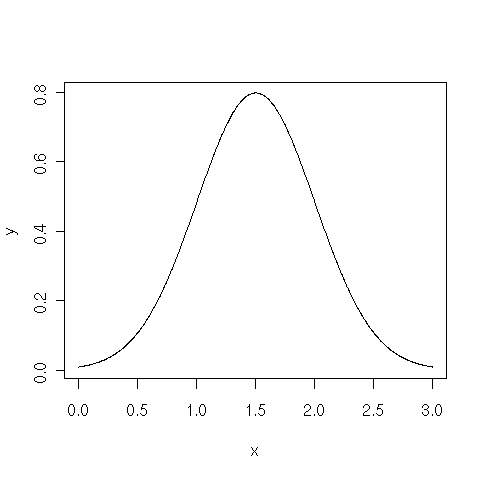
\includegraphics[scale=0.5]{chiron/normal.png}
	\end{center}
	\caption{normal}
	\label{fig:normal}
\end{figure}

\begin{figure}[h]
	\begin{center}
		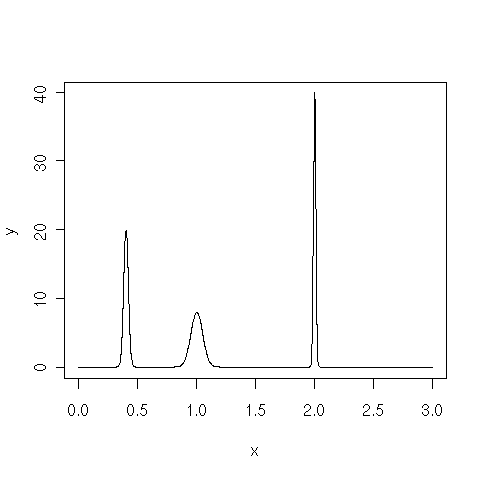
\includegraphics[scale=0.5]{chiron/pics.png}
	\end{center}
	\caption{Suma de Gaussianes difícil de trobar per Chiron} 
	\label{fig:dificil}
\end{figure} 

La solució que s'ha adoptat ha estat la de generar una població d'individus
nova, sense tenir en compte ĺa generació anterior, com si es comencés un
experiment nou.  Fent això evitem que l'algoritme genètic estigui ``viciat'' de
bon principi, i maximitzem les probabilitats de trobar algun pou d'energia
(\ref{ssub:CInicialitzacio}).

Les proves de correctesa del programa, s'han fet amb funcions matemàtiques
contínues, per tal de saber del cert que l'algorisme funciona bé i més endavant
s'ha provat amb el cas real de química combinatòria.

%Els resultats obtinguts d'aquestes funcions també seran exposats més endevant
%en l'apartat de resultats. 

\subsubsection{Testeig} % (fold)
\label{ssub:Testeig}

Hi ha un conjunt de funcions matemàtiques que es consideren ``típiques'' per a
usar-les com a ``problemes joguina'' (toy problems), per exemple, s'ha provat
l'algoritme evolutiu representant una funció on cada al·lel només té dos
possibles valors , 0 i 1, i la funció únicament suma els bits dels cromosomes.
El que es busca en aquesta funció, és maximitzar o bé minimitzar el resultat de
la suma de bits.  Aquest, tot i ser un exemple trivial, ens serveix per
saber si l'algorisme evolutiu funciona correctament.  Aquest exemple també ens
serveix perquè les mutacions i creuaments utilitzats són els mateixos que
utilitzem en la versió final de la aplicació.

Els resultats obtinguts són bons, arribant al millor resultat (tot uns) o a un
dels millors explorant només un percentatge de aproximadament el  10\% de
l'espai de cerca.

La funció de la suma de bits és una funció trivial per a qualsevol algorisme
evolutiu, donada la seva simplicitat.  És per això que després de provar amb
aquesta funció, hem provat funcions més complicades d'optimitzar, fins a arribar a
les conegudes com a ``funcions trampa''(\ref{EU2009}).  Les funcions trampa són funcions que
tenen característiques que fan molt difícil als AE trobar el màxim/mínim global,
tenint el millor resultat global envoltat de resultats molt dolents, i tenint un
màxim/mínim local ``fàcil'' d'arribar-hi en un extrem, apartant les solucions de
l'òptim global.  Una de les funcions trampa que hem provat, és la de mapejar en
un vector de bits una valoració determinada per a cada suma de bits.  Per
exemple, donat un vector de 5 posicions:

 % theme=Berlin;caption_top=1;caption=Exemple tanimotos
 % bits a 1 & valor
 % 0 & 1
 % 1 & 2
 % 2 & 3
 % 3 & 4
 % 4 & 5
 % 5 & 0

\begin{table}
\centering
\caption{Funció trampa}
\begin{tabular}{|r|r|}
\hline
\multicolumn{1}{|c|}{\textbf{bits a 1 }} & \multicolumn{1}{c|}{\textbf{ valor}} \\
\hline
\hline
0 & 1 \\
1 & 2 \\
2 & 3 \\
3 & 4 \\
4 & 5 \\
5 & 0 \\
\hline
\end{tabular}
\end{table}


L'ideal en aquest cas és trobar el vector que té 5 bits a 1, és a dir, busquem
minimitzar la funció.  Això, clarament és una trampa per a l'algorisme genètic,
ja que al fer els creuaments entre dos cromosomes que tenen una bona puntuació,
fa que els resultants, siguin molt dolents. És una manera d'enganyar al
algoritme evolutiu que ens serveix per a saber si aquest és prou robust per a
trobar un resultat bo.  En aquests casos, l'elitisme, és molt determinant per a
obtenir bons resultats.
% subsubsection Testeig (end)

%SOAP
\subsubsection{Funció fitness configurable} % (fold)
\label{ssub:Funcio fitness configurable}

Un altre aspecte important de Chiron és la versatilitat que té per a executar-se
amb diferents funcions de fitness.  Com s'ha explicat en la introducció del
capítol, Chiron permet avaluar manualment cadascun dels elements.  Donat que una
avaluació d'una molècula pot portar dies o setmanes, l'algorisme genètic ha de ser
capaç de mantenir l'estat i congelar-se a cada iteració.

Les llibreries usades (eodev), estan preparades per a mantenir l'estat en arxius
de text pla, però ho fan en el moment que s'ha acabat de executar la funció
avaluació de tots els individus d'una generació.  Per a poder aturar la
execució abans (a nivell lògic), el que hem dissenyat és un sistema per a
recollir i posar dades automàticament en els arxius de estat.  eodev està
programat en c++, i per tant, la funció de fitness ha de ser sempre la mateixa
ja que només volem tenir una instància de \texttt{Chiron} per executar, i no pas
una per a cada projecte que es faci.  El que hem fet per a solucionar aquesta
qüestió és ``anul·lar'' la funció de fitness fent que sigui una stub, que dona
fitness zero a tots els individus que avalua.  Configurant Chiron per a què
faci una sola generació, aconseguim guardar l'estat en un arxiu, amb els
paràmetres del algorisme genètic, les llavors (seed), i els individus de la
generació actual.  Llavors, el programa que executa el nucli de Chiron pot
parsejar l'arxiu, i insertar els elements en una base de dades (ens interessa
tenir un històric de tots els elements avaluats en generacions prèvies).
Aquests resultats són els que es presenten al usuari, que pot recuperar quan
vulgui ja que la recuperació de les dades es fa des de la base de dades MySql.

Quan l'usuari disposa de dades sobre les molècules, les pot introduir a través
d'una interfície, i tornar a executar una generació.

Si l'usuari ha configurat el projecte perquè mantingui els valors d'avaluacions
passades, en el moment que Chiron detecta una molècula que ja ha estat avaluada,
no li presenta al usuari, i és Chiron qui s'encarregarà de afegir el resultat en
el moment de la següent generació.

%subsub?  PRoblemes d'inicialització.

En  molts casos reals, ens trobem que tenim una immensa majoria de valors iguals
com a resultat de les avaluacions.  Aquests resultats són per les molècules que
o bé no poden ser sintetitzades, o bé no superen un llindar mínim d'activitat.
La manera com hem solucionat aquest problema s'explica detalladament en
l'apartat \ref{ssub:CInicialitzacio}.

% subsubsection Funció fitness configurable (end)

%BBDD
\subsubsection{Emmagatzematge de les dades} % (fold)
\label{ssub:Emmagatzematge de les dades}

Per a guardar l'estat del procés, hem creat una base de dades que ens permet
accedir i modificar la informació de un projecte.  La implementació d'aquesta
base de dades la hem fet amb MySql (més endavant es discutirà el perquè de la
elecció d'aquesta tecnologia en front a altres bases de dades, o altres
tècniques per a emmagatzemar dades (com poden ser Tokyo Cabinet/Tyrant, MongoDB
o altres SGBDs orientats a Documents,o diccionaris clau-valor).

\lstset{language=sql, tabsize=2}
\lstset{commentstyle=\textit}
\lstinputlisting[frame=trbl]{chirondb.sql}

Aquesta estructura ens permet tenir un historial de tots els elements que han
anat construint-se en els diferents experiments per a futurs anàlisis i
visualitzacions.
% subsubsection Emmagatematge de les dades (end)

\subsubsection{Webservice d'algorismes genètics} % (fold)
\label{ssub:Webservice d'algorismes genetics}

%SaaS WEB i SOAP
Una vegada tenim desacoblats el nucli (algoritme evolutiu), de la base de dades,
i del wrapper que va executant el nucli sobre els diferents projectes, i gestiona
la base de dades, ja tenim un programa funcional, que ens permet fer el que
volem.  Però encara tenim l'impediment de la interfície.  Un programa amb
múltiples usuaris, pensat per a solucionar problemes molt diferents entre si
(sempre pensant amb la química combinatòria com a funcionalitat principal,
 però intentant generalitzar i aconseguir la màxima abstracció possible), hauria
de tenir una interfície que permeti la execució del programa des de punts
diferents de un procés i des de diferents interfícies (front-ends).

Pensant amb la química combinatòria, la aplicació s'ha pensat des
d'un principi amb una interfície web en ment.  Per això, com a objectiu
principal, la interfície que fem a Chiron ha de permetre l'accés web.  Una
interfície web permet al usuari connectar-se des de on vulgui, sempre i quan
tingui accés a la xarxa, i un usuari habilitat.  Un avantatge clar de les
interfícies web és que l'usuari no haurà d'instal·lar cap programari per a executar
Chiron.  Per als interessos comercials d'Intelligent Pharma, també ha estat un
punt important, ja que l'usuari  final (client), pot rebre actualitzacions i
millores sense haver de fer res en absolut, sinó que tot el control recau sobre
el distribuïdor del programa.

Altres avantatges d'utilitzar un model de negoci ``Software as a Service''
(SaaS) és que el control del software recau sobre el distribuïdor, no només en
termes de actualitzacions i seguretat, sinó que obre noves possibilitats en
termes de models de pagament.   Per exemple, al no distribuir un software,
s'elimina la possibilitat de violacions de contracte o còpies il·legals, ja que
l'usuari no disposa mai del software, fent impossible la còpia, o l'ús
fraudulent d'aquest.  Les estadístiques que pot treure el distribuïdor (complint
els contractes de privacitat, és clar), son molt més potents que els clàssics
``bug reports'', podent acurar molt més el producte a les necessitats dels
usuaris, ja que sabent quines funcionalitats utilitzen més, o bé quins workflows
segueixen, podem tenir indicis de què i com s'ha de millorar.

Aquesta tendència del SaaS, està essent molt utilitzada en els darrers anys en
front al clàssic software instal·lat al client ja que, amb l'augment d'importància
del Cloud computing, i les tecnologies distribuïdes (Grid, globus, web 2.0), la
idea és que l'usuari d'un producte, sigui únicament això, un usuari d'un servei,
però no hagi de tenir cap coneixement ni infrastructura prèvia per a
utilitzar-lo.

SaaS també ha despertat dubtes i queixes, bàsicament en dues vessants:

Una d'elles és la dependència en el proveïdor de software.  No tenir cap tipus
d'infrastructura, suposa estar en mans del proveïdor, i per tant, si els
servidors del proveïdor no funcionen bé, o hi ha problemes d'accés, l'usuari
no controla les dades, ni pot fer res més que posar-se en contacte amb el
proveïdor del servei.  Aquesta falta d'autosuficiència fa que encara generi
desconfiança en certs sectors.

La privacitat també és un altre punt on s'ha generat certa desconfiança.  Les
dades, tot i que són accessibles per l'usuari, estan emmagatzemades en els
servidors del proveïdor.  Tot i que la legislació és molt clara al respecte,
hi ha clients que desconfien.

%WEB
Per altra banda, el testeig i la automatització de procediments a través de la
web és difícil per definició (no té estat, i les maneres més ``sofisticades''
per interactuar amb elles són macros no gaire intel·ligents).

Si només proporcionéssim interfície web, Chiron estaria sempre supeditat a la
utilització interactiva amb un usuari a l'altra banda.  Tot i que per Chiron, ja
serviria, hem de pensar en línies de futures aplicacions.  És per això que la
web no es comunica amb Chiron directament, sinó que hem programat una interfície
per a execució remota, i la web es comunica amb la interfície intermitja.

Aquesta interfície intermitja ens dóna la funcionalitat de poder accedir al
nucli de Chiron a través de programes, convertint Chiron en un servidor 
d'algoritmes genètics.

%Client-servidor. explicar una mica de que va el paradigma
Per a implementar el servidor de aplicacions remotes, s'han estudiat diverses
opcions, i ens hem decantat per a implementar una interfície SOAP.  Tot seguit
es discutiran les diferents opcions, i el perquè de la elecció, i en l'apartat
de implementació, es detallarà més la implementació de SOAP, i el funcionament
intern d'aquest.

%Execució remota
%RMI
%CORBA
%REST
%XML-RPC
%SOAP

Per a convertir Chiron en un servidor de algorismes genètics, que sigui usable
tant per persones (a traves de la web) com per aplicacions que connectin una
funció de fitness definida per elles al algorisme genètic, hem estudiat diverses
opcions, que analitzarem per sobre (donant algunes referències bàsiques).

L'objectiu és trobar una tecnologia que permeti fer crides remotes a un servidor
de funcions.  Com que el control del estat del programa el tractem manualment
(base de dades, etc) no necessitem que el sistema ens guardi la persistència.
Si utilitzéssim un sistema així també tindríem problemes a la hora de aturar el
servidor, i hauríem de crear un sistema de backups, amb lo que no ens
estalviaria la feina.

Necessitem doncs, exposar al exterior un conjunt de funcions aïllades, seguint el
paradigma client-servidor, que siguin extensibles i interpolables entre
diferents llenguatges de programació. Es pot veure la estructura de la
comunicació entre els processos en la figura \ref{fig:401px-Orb.png}.

\begin{figure}[h]
\centering
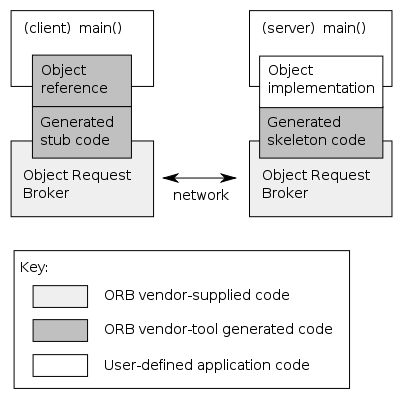
\includegraphics[scale=0.5]{401px-Orb.png}
\caption{Model de Client-servidor que necesitem}
\label{fig:401px-Orb.png}
\end{figure} 

Tecnologíes per a executar RPCs (Remote procedure call) n'hi ha moltes
diferents. Les tecnologies que ens obliguen a utilitzar el mateix llenguatge de
programació han quedat descartades de bon principi, ja que un dels objectius
principals és precisament obrir el programa a futures aplicacions que puguem
crear.  És per això que RMI, que ens lliga a java no pot ser utilitzada.  

Una altra alternativa que hem estudiat és CORBA, que és un sistema molt extès
per a tipus d'aplicacions client-servidor en xarxa, i proporciona una capa
intermitja molt còmoda i extensible.  CORBA és un sistema dissenyat per a
comunicar diferents llenguatges entre si.  Per aquesta part, ens serveix per als
nostres requeriments, però el protocol de CORBA funciona utilitzant ports TCP
no estàndards, i fa que no puguem garantir la connectivitat si el client o bé el
servidor estan darrere d'un tallafocs (firewall).

La aplicació Chiron ha de funcionar a través d'una interfície web que estarà
allotjada en un servidor local, i nosaltres controlem la xarxa, però com que
part de la essència de Chiron és el sistema de algorismes genètics genèric, no
volem limitar-nos a la utilització únicament per web.  Per això, s'han seguit
buscant alternatives.

Per assegurar que no tenim bloquejos en la xarxa, hi ha sistemes dissenyats per a
treballar només a través de ports coneguts, i normalment oberts en qualsevol
xarxa amb connexió a internet.  Exemples d'aquestes tecnologies son XML-RPC, REST
i SOAP.
% subsubsection Webservice d'Algorismes genètics (end)

\subsubsection{Disseny global} % (fold)
\label{ssub:Diseny global}

Després de diverses iteracions sobre el disseny, la estructura global que ha
quedat del projecte \texttt{Chiron} és la mostrada en la Figura \ref{fig:disenyChiron}.

Chiron es pot integrar en altres programes ja existents de l'empresa, donant
suport amb els algoritmes evolutius.  
%(XXX: El diagrama s'ha de fer més específic per a Chiron).

\begin{figure}[h]
	\begin{center}
		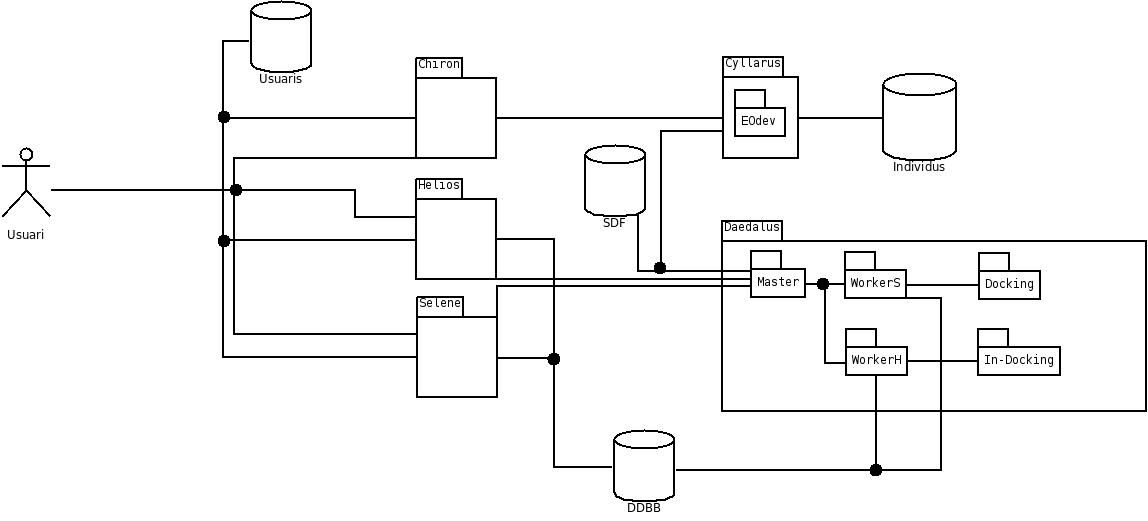
\includegraphics[scale=0.4]{chiron/arquitectura_global_chiron.jpg}
	\end{center}
	\caption{Es}
	\label{fig:disenyChiron}
\end{figure}
% subsubsection Diseny global (end)

% subsection Funcionament General (end)

\subsection{Algoritme Genètic} % (fold)
	\label{sub:Algoritme Genetic}
% subsection Algoritme Genetic (end)

L'algorisme genètic de Chiron, és un algorisme a ``mig implementar'', en el
sentit que  al ser parametritzable en quant a la funció de fitness, li falta una
de les parts principals dels algorismes genètics.  Això no vol dir que no haguem
implementat la funció de fitness, sinó queda externalitzada respecte el nucli de
\texttt{Chiron}.  Tot seguit s'explica la implementació de cadascun dels
paràmetres i estructures de dades necessàries per a la implementació de Chiron.

\subsubsection{Inicialització} % (fold)
\label{ssub:CInicialitzacio}

En  molts casos reals, ens trobem que tenim una immensa majoria de valors iguals
com a resultat de les avaluacions.  Aquests resultats són per les molècules que
o bé no poden ser sintetitzades, o bé no superen un llindar mínim d'activitat.

Això ens ha suposat un gran problema perquè si avaluem la primera generació i
tots els elements tenen el mateix fitness (0), la següent població que Chiron
suggerirà serà una població tal que haurà sortit de creuar i mutar la primera
població aleatòriament entre ella.  Aquest procediment ens provoca una
convergència prematura que no desitgem, ja que el que passa en realitat és que
encara no hem mostrejat cap molècula que ens doni un mínim d'activitat amb el
que poder ``jugar''.

Problemes d'aquestes característiques només es donen en casos on l'espai de
cerca és molt gran comparat amb el número de elements que tenen resultats
diferents de 0.

Per exemple, si volguéssim trobar, en el problema de la suma de bits una
configuració concreta (10101), o bé trobar elements amb unes certes
característiques (que sumin 3), i tots els elements que ho compleixen tenen
fitness 1 i els que no, tenen fitness 0, ens trobaríem amb problemes similars.

Aquest problema, l'hem solucionat provocant que Chiron resetegi l'experiment
(recordant les molècules avaluades en la base de dades), i torni a donar una
població d'individus aleatòria.  Així maximitzem les probabilitats de trobar un
o més pous energètics, que son les àrees del espai de búsqueda (normalment
contínues) on es troben els elements amb fitness superiors al llindar.  En el
moment que trobem molècules amb activitat, l'algorisme segueix el procediment
normal.

% subsubsection Inicialització (end)

\subsubsection{Individu (Cromosoma)}
\label{ssub:individu (cromosoma)}

En aquest algorisme genètic, els indicis són les diferents combinacions de
ramificacions, en cadascuna de les posicions. Com que els canvis entre un al·lel i un
altre són qualitatius, cada posició del cromosoma és un enter, que representa
una terminació diferent en funció de la posició on es troba dins el cromosoma.

Així doncs, tenim un vector de N posicions on N és el número de ramificacions que té
l'esquelet, i cada posició conté un enter, amb límits d'acord amb les
especificacions del usuari al iniciar el projecte. 

Utilitzem enters per a representar cada al·lel perquè és la forma més còmoda que
tenim per representar valors qualitatius o categòrics.  A més, els valors límit
de cada posició s'acoten en cada projecte.  Això és un altre tret que el
diferència de programes més estàtics on els límits són coneguts a priori, com
per exemple Pholus (\ref{cha:Pholus}).

Si els possibles valors adoptats en cada punt fossin coneguts en temps de
desenvolupament del projecte, es podria usar tipus enumerats, per a deixar ben
clar que els valors són qualitatius i que hi ha la mateixa diferència en un
al·lel entre el valor 1 i el 2 que entre el 1 i el 5, ja que simplement són
ramificacions diferents, i no tenen res a veure un amb l'altre.  Això també ens
condiciona els creuaments, com s'explica en la següent secció.

%PUNT

\subsubsection{Selecció} % (fold)
\label{ssub:CSeleccio}
En aquest problema, hem utilitzat un algorisme de sel·lecció per Torneig
determinista ($p=1$), on competeixen dos individus.  Donat que les poblacions
són relativament petites en la majoria de casos (tenim un espai total de cerca
de gairebé 16000), hem utilitzat un torneig petit, ja que la pressió evolutiva
que implica pujar el torneig en un és molt gran, i de seguida ens estanca en
problemes de convergència prematura.

% subsubsection Selecció (end)

\subsubsection{Creuament} % (fold)
\label{ssub:Crossover}

Com a operador de creuament entre 2 individus d'una generació, s'utilitza el
tall per 1 punt.  La raó d'això és que cadascun dels al·lels té un valor
qualitatiu, i no té cap sentit fer altres creuaments on el mateix gen (mateixa
posició del vector) es creua físicament amb el gen de l'altre cromosoma.

Un creuament que involucrés aritmètica no es pot fer servir en aquest cas ja que
no es poden sumar ``peres i pomes''.

Creuaments que involucrin el canvi de posició en els gens tampoc eren naturals
per aquest problema, ja que s'hauria de comprovar que cap gen es col·loca en una
posició on no pot ser-hi ja que supera els límits estipulats per la
posició final.  A part d'aquest fet totalment subjecte a implementació, i per
tant, solucionable amb una mica més de comprovacions, aquests creuaments no
tenen sentit químic, ja que l'alternativa $i$ de la posició $n$, no té perquè
tenir res a veure, ni cap correlació amb l'alternativa $i$ de la posició $m$ on
$n <> m$.

Pel creuament s'ha provat un creuament per un punt, i el creuament per dos
punts, donant resultats similars en els dos casos.  Donat que els experiments
químics en què s'ha provat (\ref{sec:Resultats}), tenen només tres llocs per a
substituents, un creuament per diversos punts no tenia gaire sentit.

Donats dos individus (els que han estat sel·leccionats en el procés de
sel·lecció per a reproduir-se , amb una probabilitat d'un 0.8 es fa creuament i
els fills són tan sols una partició formada a partir dels 2 pares, amb un punt
de tall aleatori.  Donat que no hi ha cap relació entre els diferents indexos
(estan ordenats arbitràriament) no ens hem de preocupar de partir el cromosoma
per lloc ``delicat''. 

Així doncs, el que es busca és interpolar les qualitats de dos individus ben
adaptats, per a crear uns descendents amb propietats similars.  És d'esperar que
si un individu té bon fitness, les ponderacions donades als seus indicadors
siguin bastant encertades.  Llavors, en interpolar una parella de individus,
suposem que el descendent també tindrà un fitness bo, i això farà que a mesura
que passen les generacions, la població tendeixi a millorar (en mitja).

En els experiments en formules matemàtiques, ha donat millors resultats el tall
en 2 punts, que no pas en 1.

% subsubsection crossover (end)

\subsubsection{Mutacions} % (fold)
\label{ssub:Mutacions}

La única mutació que té sentit en aquest problema és canviar un dels elements
del cromosoma per un altre, sempre dins del rang que tingui en aquesta posició.

Intercanvis de al·lels de diferents posicions no són possibles ja que les
diferents posicions del cromosoma tenen rangs diferents, i fa que molts dels
intercanvis que faríem siguin invàlids.
% subsubsection Mutacions (end)


\subsection{Implementació} % (fold)
	\label{sub:Implementacio}

Tot seguit es detallen algunes particularitats de la implementació de
\texttt{Chiron}, amb les seves tecnologies, i algun codi exemplificador del que
s'està explicant.

\subsubsection{Algorisme genètic} % (fold)
\label{ssub:algorisme genetic}

En aquest projecte s'han utilitzat les llibreries eodev, igual que en el
projecte \texttt{Pholus}, ja que ens proporcionen les qualitats suficients per a
poder treballar per sobre d'elles sense haver de fer gaires modificacions sobre
el seu codi base.

Eodev proporciona una estructura genèrica per a algorismes genètics, on, si no
volem massa complicacions, amb un cromosoma de coma flotants, modificant només
la funció de fitness, podem corre ja el nostre algorisme genètic.  Això no ens
serveix per a \texttt{Chiron}, ja que necessitem modificar el cromosoma, les
mutacions i creuaments per al que volem fer nosaltres.

Hem de crear doncs, una classe per a cada element del algorisme genètic.

%PUNT posar totes les classes

% subsubsection algorisme genètic (end)

\subsubsection{Arxius de configuració} % (fold)
\label{ssub:Arxius de configuracio}

Eodev disposa d'una manera per llançar execucions amb un arxiu de configuració
determinat.  El format no respon a cap estàndard (ni .ini, ni .conf\ldots).
Aquest format és el que fem servir per a llançar procéssos \texttt{Chiron}, amb
els parametres adequats, i per altra banda, entre generació i generació, omplim
els fitness en l'arxiu aquest.  És una manera de colar-se en el procediment de
Chiron, i permetent-nos modificar el fitness d'un element en una generació
determinada.

Per a generar aquest arxiu de configuració hem agafat un dels de demostració que
vénen amb les fonts de Eodev, i hem creat un template o plantilla, utilitzant
Template Toolkit (TT\footnote{\url{http://template-toolkit.org/}}).
\cite{CCW03}.

Template Toolkit és una llibreria molt estesa per a la generació de textos
parametritzats.  En un principi es va crear per a reproduir textos massivament,
on només canvia una petita part del text (per exemple, circulars), o bé arxius
que han de complir una certa estructura (webs corporatives).

Nostres hem usat la implementació en Perl, que a part de ser la primera que va
sortir (i potser la més sòlida), és el llenguatge en el que hem desenvolupat
tota la part que no forma part del nucli de la aplicació.  Segueix un exemple de
la utilització de Template Toolkit en un cas senzill, i la manera en que ens
facilita la separació de la presentació de la lògica.  És per això que Template
Toolkit també s'utilitza en molts frameworks web perl\footnote{Catalyst.
http://www.catalystframework.org/}.

%codi Template Toolkit
\lstset{language=perl, tabsize=2}
\lstset{commentstyle=\textit}
\lstinputlisting[frame=trbl]{tt.pl}

Encara que en aquest exemple, no sembla més que una versió ``més elegant'' de
sprintf, Template Toolkit pot afegir lògica en les seves plantilles, processant
o no processant arxius en subdirectoris, en funció de valors de variables en el
programa perl que crida les funcions TT.

% subsubsection Arxius de configuració (end)

\subsubsection{DBIx::Class} % (fold)
\label{ssub:DBIx Class}

Tant l'arxiu de configuració de cada projecte, com la informació dels individus
que han aparegut en generacions passades del projecte, i com el propietari de
cada projecte es mantenen en una base de dades MySql.

La decisió de MySql o bé PosgreSql, no ha estat una decisió on hi hagi hagut un
clar guanyador.  Pel volum de dades que hem de tenir, tampoc creiem que això
sigui una decisió critica per al èxit del projecte, però per si de cas, hem
decidit utilitzar un sistema de ORM \footnote{Object Relational Mapper} .

Els ORMs són llibreries que mapegen taules SQL a objectes del llenguatge, podent
així fer més directe el tractament amb bases de dades des de llenguatges de
programació, fent que no s'hagi de fer un canvi de paradigma tant gran al
canviar de OOP pura a \texttt{SELECT * FROM \ldots}.

Sabem doncs, que per al projecte, en l'estat actual no és necessari plantejar-se
quina és la millor base de dades a escollir, si hem fet una bona elecció pel
que fa a les eines i llibreries, ja que utilitzant DBIx::Class, canviar de SGBD no
suposa cap modificació en el codi, fent-ho del tot transparent.

% subsubsection DBIx\dots Class (end)

\subsubsection{Webservices i Soap} % (fold)
\label{ssub:WS i Soap}

Com ja s'ha explicat anteriorment (\ref{sec:Procediment informatic} ), per a la
comunicació segons el paradigma client-servidor, s'ha utilitzat la tecnologia
SOAP\footnote{Simple Object Access Protocol}.

Els seus rivals més igualats, per als nostres requeriments, han estat XML-RPC i
REST, però hem decidit utilitzar SOAP, entre d'altres coses, perquè és l'únic
que té suport a nivell corporatiu, i no com REST, que son estàndards
desenvolupats majoritàriament en entorns de comunitats Opensource.  Al
utilitzar-lo nosaltres en un entorn corporatiu, hem pensat que SOAP seria més
adequat pel possible suport que tindria i la interpolabilitat amb altres
aplicacions que es poden utilitzar en el futur.
%PUNT . POSAR L'ESTANDARD SOAP, I WSDLs i XMLs d'exemple?

% subsubsection Webservices i Soap(end)
% subsection Implementació (end)
% section Procediment informàtic (end)

\section{Resultats} % (fold)
	\label{sec:Resultats}

	En les proves que hem realitzat, \texttt{Chiron} ha donat bons resultats,
	però necessitem fer algunes validacions per a assegurar que ha valgut la
	pena aquest esforç, i també tenir dades objectives sobre la seva utilitat.
	A nivell comercial, també es vol tenir alguna validació estadística que ens
	doni seguretat per a ``vendre'' Chiron.

	Per a realitzar les proves inicials, s'han utilitzat funcions típiques de
	testeig d'algorismes genètics, com la suma de bits (es tracta de maximitzar
	el número de bits a 1 en un vector), o alguna funció trampa, on el màxim de
	la funció no està en cap extrem del espai de búsqueda.

	Les proves sobre un escenari real en el que operarà Chiron, s'han fet sobre
	tres projectes dels quals s'ha realitzat la prova experimental de totes les
	combinacions de substituents possibles (s'han trobat en (XXX Ppaper) )

	En aquests tres problemes, els autors dels experiments van sintetitzar totes
	les possibles molècules, obtenint un resultat de activitat en cadascuna
	d'elles.  És possible que algunes d'elles fossin impossibles de sintetitzar,
	i que els hi haguessin posat un fitness molt baix.  Això ja ens va bé per
	als nostres propòsits, ja que és el mateix resultat que els hi donaríem
	nosaltres.

	Per a testejar Chiron, hem usat un programa de test, que analitza totes les
	dades experimentals, tenint així una resposta per a cada possible individuu
	que pugui proposar Chiron.

	Aquest programa de prova, ha estat desenvolupat en Perl, atacant directament
	la llibreria també programada en perl, no pas usant la interfície SOAP, ja
	que podent fer les proves en local, és molt més ràpid en executar-se.

	S'han fet 25 execucions de Chiron per a cada projecte, i hem
	esperat a què convergeixin cadascun dels 3 projectes.  Com que tenim a la
	nostra disposició totes les dades del espai de cerca, hem fet càlculs
	respecte quantes avaluacions s'han fet fins a trobar el millor element que
	hem arribat a trobar.  També ens fa falta saber quin és el fitness d'aquest
	element, i quin és el fitness de la millor combinació de substituents que
	hi ha en tot l'espai de cerca. 

	%TAULA de resultats.

% theme=Berlin;caption_top=1;caption=Exemple tanimotos
% BBDD & Fitness & Elements avaluats & relació

%png('file.png')
%hist(x)
%dev.off()

	En les figures \ref{fig:resChir1},\ref{fig:resChir2} i \ref{fig:resChir2} es
	mostren les validacions que s'han fet a Chiron.  

	\begin{figure}[tbp]
		\begin{center}
			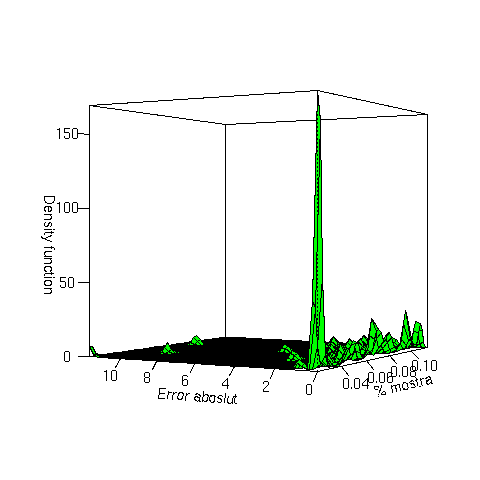
\includegraphics[scale=0.75]{chiron/rgrau1.png}
		\end{center}
		\caption{Resultat Chiron 1}
		\label{fig:resChir1}
	\end{figure}

	\begin{figure}[tbp]
		\begin{center}
			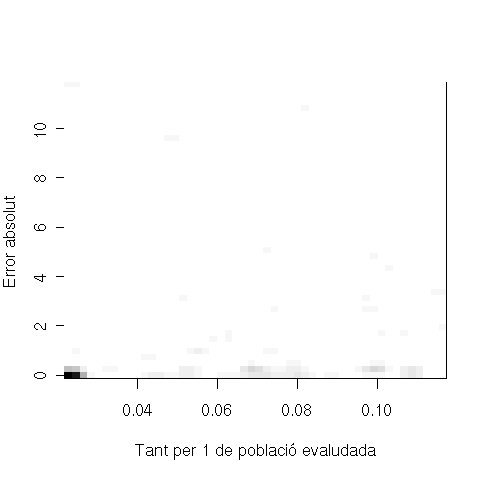
\includegraphics[scale=0.75]{chiron/GraficaChironGuai.png}
		\end{center}
		\caption{Resultat Chiron 2}
		\label{fig:resChir2}
	\end{figure}

	\begin{figure}[tbp]
		\begin{center}
			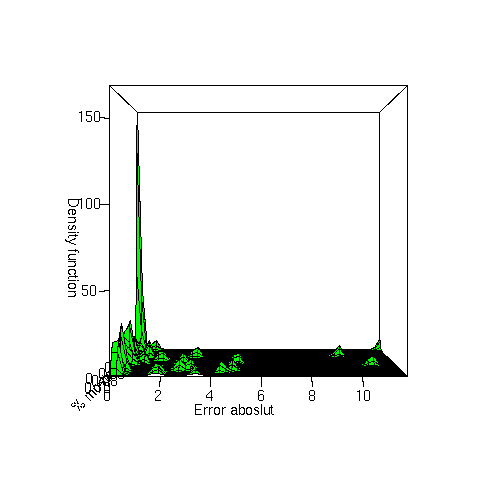
\includegraphics[scale=0.75]{chiron/rgrau3.png}
		\end{center}
		\caption{Resultat Chiron 3}
		\label{fig:resChir3}
	\end{figure}
	\begin{figure}[tbp]
		\begin{center}
			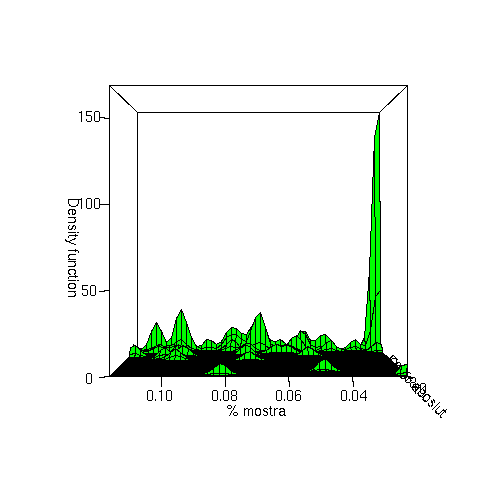
\includegraphics[scale=0.75]{chiron/rgrau4.png}
		\end{center}
		\caption{Resultat Chiron 3}
		\label{fig:resChir4}
	\end{figure}

	Aquestes gràfiques mostren, de diferents maneres, el nombre de elements
	avaluats, i l'error absolut que s'ha obtingut en cadascun dels experiments.

	La intenció inicial era utilitzar l'error relatiu, però en aquests
	experiments, els pitjors fitness tenen un valor de infinit.  Com que els
	tres experiments sobre els que hem fet les proves són molt similars en quant
	al millor fitness possible (0, 0.1 i 0.09), hem pogut dissenyar un
	sistema de tests unificant els resultats dels tres experiments, i així tenir
	una idea més general del rendiment de \texttt{Chiron}.

	Com ja s'ha dit prèviament, s'han  realitzat 25 execucions de cadascun dels
	tres experiments, guardant per a cadascun el número d'individus que s'han
	avaluat, el número total d'individus del espai de cerca, el millor fitness
	de tot l'espai de cerca, i el millor fitness al que hem arribat.

	D'aquesta manera, hem pogut fer un estudi estadístic sobre el funcionament i
	rendiment de Chiron.

	L'estudi, estadístic, l'hem realitzat utilitzant el software estadístic
	R(\url{http://www.r-project.org/}), i ens permet dir coses com per exemple, que \textbf{avaluant un XXX
	\% de l'espai de búsqueda, ens quedem a XXX del millor en un XXX dels casos}


\section{Conclusions i treball futur} % (fold)
\label{sec:CConclusions i treball futur}

	Amb tot el desenvolupament i proves realitzades, hem assolit l'objectiu
	d'aquesta part del PFC.  Tot i això com a projecte futur
	d'ampliació, està implementar tècniques de algorismes genètics interactius.

	Donat que la avaluació és supervisada per l'usuari, podríem implementar
	tècniques per a classificar els individus de cadascuna de les generacions,
	per a només donar al usuari una part de la població a avaluar, en funció de
	la semblança entre els individus.  Es podria utilitzar alguna tècnica de
	clustering, o eines més particulars d'algorismes genètics interactius.
	% subsection treball futur (end)
% section Resultats (end)

%\end{document}
%# vim: set tabstop=4 shiftwidth=4 tw=80 foldmethod=marker ignorecase : ##


% chapter Chiron (end)



\chapter{GEP} % (fold)
\label{cha:GEP}
% chapter GEP (end)

%Resultats del PFC (números i exemples)
\chapter{Resultats}
	%\include{resultats}

%Conclusions del PFC
\chapter{Conclusions\label{chap:conclusions}}
	%\chapter{Conclusions} % (fold)
\label{cha:Conclusions}

En la realització d'aquest projecte de final de carrera, s'ha desenvolupat un
conjunt d'eines que permeten millorar la efectivitat real dels processos de
descobriment de nous fàrmacs aplicant algoritmes evolutius amb èxit.
Aquests programes, són eines que no funcionen aïllades, sinó que milloren
processos intermedis que amb les eines disponibles fins al moment, no es feien
tan eficientment, o bé simplement, no existien eines per a tractar aquests
problemes.

Del conjunt d'experiències adquirides en aquest projecte, podem treure diverses
conclusions  Segueixen les tres que resumeixen millor els valors apresos de la
realització d'aquest PFC.

\begin{itemize}
	\item Les eines d'intel·ligència artificial, poden aportar millores reals a
		les metodologies existents avui en dia per a la recerca de nous fàrmacs.
	\item Concretament, els algorismes evolutius han demostrat un cop més que poden ser molt eficaços i competitius en grans espais de cerca, entorns amb difícil avaluació de les potencials solucions i problemes complexos i epistàtics, com els tres problemes on s'ha treballat.
	\item Els programes que creem, han de tenir una interfície adequada, no
		només cap als usuaris finals, sinó que s'han de fer, en la mesura del
		possible reutilitzables, i accessibles des d'altres programes.
		Tecnologies basades en webservices són molt útils per aquestes tasques.
	\item Hofstadter's Law: It always takes longer than you expect, even when
		you take into account Hofstadter's Law \cite{GEB79}.
\end{itemize}

A nivell d'acceptació comercial els tres projectes \texttt{Pholus, Chiron i GEP}
han corregut una sort diferent, que també és interessant fer notar.

\paragraph{Pholus} % (fold)
\label{par:Pholus}

Pholus, ha estat un èxit rotund, i s'està utilitzant actualment en el procés de
HELIOS (Intelligent Pharma), utilitzant-se per extensió en la majoria dels laboratoris
farmacèutics d'Espanya.  És per això que aquest projecte ha sofert diverses
ampliacions i modificacions, de les que no hem parlat en aquest projecte, però
que ens donen una idea del moviment i la utilització que ha sofert aquest
programa. De fet, Pholus està sent utilitzat en aquests moments en una quinzena de projectes de recerca diferents, en àrees terapèutiques tan diverses com oncologia, cardiovascular, hematologia, antibiòtics, etc.

Tot i que l'algorisme evolutiu que hi ha dins de Pholus és aparentment senzill,
molta complexitat ve donada pel context químic en el que es troba.
% paragraph Pholus (end)

\paragraph{Chiron} % (fold)
\label{par:Chiron}

Per la seva part, Chiron és un projecte en estat embrionari, tot i que s'ha testejat amb èxit en alguns problemes reals, la seva comercialització no ha estat massiva.
Per altra banda, Chiron ha estat pensat per a ser un webservice d'algorismes genètics,
i es pot enllaçar amb altres programes, que aporten a Chiron la funció de
avaluació.  Aquest projecte ha requerit el domini de moltes tecnologies
diferents, i ha estat un molt bon exercici d'integració d'eines
(c++, perl, mysql, SOAP, php).
% paragraph Chiron (end)

\paragraph{GEP} % (fold)
\label{par:GEP}
GEP ha estat el projecte que ha tingut menys ``sort'', tot i ser molt
interessant pel grau de recerca bàsica que comporta.  Aquesta evolució de la programació genètica no ens ha permès solucionar els problemes pels que havíem pensat utilitzar-ho, degut a que les funcions que volíem trobar (periòdiques) afegien
dificultat al problema, i tant la falta de temps, com alternatives que s'han
trobat en l'empresa, han fet que no s'investigués més a fons.  De totes maneres,
hem aconseguit resultats similars als últims articles apareguts en la matèria,
en funcions polinòmiques.  Treballar amb tècniques totalment noves (els primers
articles daten de 2001 \cite{ferreira:2001}) ha sigut una experiència molt
estimulant.
% paragraph GEP (end)
\\ 
\\

Concloem doncs que els algorismes evolutius s'adapten molt bé a la resolució dels tres problemes abordats, que s'han aportat innovacions tècniques importants pel descobriment de nous fàrmacs i amb una gran repercussió industrial, i que el treball en equips de recerca interdisciplinària és estimulant però a l'hora complex en les comunicacions.

% chapter Conclusions (end)

%\section{Programari utilitzat i repositoris} % (fold)
%\label{sec:Programari utilitzat}

%Per a la realització d'aquesta memòria, s'ha utilitzat \latex, vim, emacs, R i
%the gimp.  Tot el software utilitzat és software lliure.  Aquest document es pot
%trobar a \url{http://github.com/kidd/pfc}. 
%% section Programari utilitzat (end)


\appendix 
\chapter{Fitxers AutoDock}
	%\include{autoDockFiles}
\chapter{Codis font}
	%\include{codis}

\bibliography{bibliography}
\bibliographystyle{unsrt}
\end{document}


%%% Local Variables:
%%% mode: latex
%%% ispell-local-dictionary: "catala-tex"
%%% End:
